\documentclass[]{foi}

\usepackage[utf8]{inputenc}

\usepackage{graphicx}
\usepackage{array}
\usepackage{makecell}
\usepackage{booktabs}
\usepackage{caption}
\usepackage{float}
\usepackage{lipsum}
\usepackage{fvextra}
\usepackage{lineno}
\usepackage{csquotes}
\usepackage{hyperref}
\usepackage{enumitem}
\usepackage[table]{xcolor}
\usepackage{tabularx}
\usepackage{tcolorbox}
\usepackage{listings}
\usepackage{minted}
\newcolumntype{R}[1]{>{\raggedright\arraybackslash}p{#1}}



% Definicija boja
\definecolor{lightgray}{gray}{0.97}
\definecolor{darkblue}{rgb}{0.1,0.1,0.6}
\definecolor{darkgreen}{rgb}{0.0,0.5,0.0}
\definecolor{orange}{rgb}{1.0,0.5,0.0}
\definecolor{purple}{rgb}{0.6,0.0,0.6}
\definecolor{keywordpurple}{rgb}{0.5,0.0,0.5}
\definecolor{codebg}{rgb}{0.95,0.95,0.95}


\lstset{
  backgroundcolor=\color{lightgray},
  basicstyle=\ttfamily\footnotesize,
  frame=single,
  breaklines=true,
  numbers=left,
  numberstyle=\tiny\color{gray},
  showstringspaces=false,
  escapeinside={(*@}{@*)}, 
  keywordstyle=\color{keywordpurple}\bfseries,
  commentstyle=\color{darkgreen}\itshape,
  stringstyle=\color{orange},
  morekeywords={
    const, let, var, function, return, import, from, export, default,
    useState, useEffect, className, if, else, map, render, async, await,
    props, setState, onClick, true, false
  },
  captionpos=b
}


\renewcommand{\arraystretch}{1.3}
\setlength{\tabcolsep}{8pt}  


\geometry{margin=2.5cm}
\vrstaRada{\diplomski}

\title{Informativna platforma s inteligentnim asistentom o Erasmus+ iskustvu u \L\'{o}d\'{z}u}

\predmet{}

\author{Aleksandar Babić} 

\spolStudenta{\musko} 

\mentor{Bogdan Okreša Đurić}

\spolMentora{\musko} 

\titulaProfesora{doc.~dr.~sc.}

\godina{2025}
\mjesec{rujan}

\indeks{0016147642}

\smjer{Baze podataka i baze znanja}

\sazetak{Teoretski dio rada istražuje studiranje kao važan segment u životnom razdoblju pojedinca te se dotiče razmjene studenata u svrhu Erasmus+ studijskog boravka. 
Teoretski dio završava poglavljem posvećenim inteligentnim asistentima temeljenima na RAG (eng. Retrieval-Augmented Generation) tehnologiji.
Praktični dio rada obuhvaća izradu web-stranice s tematikom Erasmusa+ studijskog boravka i izradu inteligentnog asistenta, pri čemu je iskorišten postojeći jezični model. 
To podrazumijeva treniranje i prilagođavanje specifičnom skupu podataka, kako bi se osiguralo da inteligentni asistent odgovara upitima korisnika i pruža relevantne informacije.
}

\kljucneRijeci{Inteligentni asistent, RAG, web stranica, studiranje, Erasmus+, umjetna inteligencija.}

%\acrodef{VAS}{višeagentni sustav}


\begin{document}

\maketitle

\tableofcontents

\makeatletter \def\@dotsep{4.5} \makeatother
\pagestyle{plain}



\chapter{Uvod}

Na početku rada obrađuje se pojam studiranja kao i svi aspekti koji se usko vežu uz njega. Poseban naglasak je stavljen na važnost studiranja u kontekstu osobnog razvoja, izgradnje karaktera
te stjecanja različitih znanja. U nastavku se detaljnije razmatra Erasmus+ program, s ciljem približavanja njegovih mogućnosti i koristi. Glavni cilj je ukazati na izazove poput nedostatka interesa
za prijavu na Erasmus+ studijski boravak, prisutnog straha, nesigurnosti te neinformiranosti među studentima. 

Kao rješenje na navedene izazove izrađena je web stranica s inteligentnim asistentom koji je namijenjen da odgovori na specifične upite korisnika. Web stranica predstavlja sredstvo informiranja 
prvotno za sve studente koji dolaze u Łódź iz svojih država. Osim toga web stranica je naravno dostupna i namijenjena i za sve ostale zainteresirane posjetitelje. Web stranica se sastoji od 
početne stranice, stranice koja opisuje kratko Łódź, stranice koja prikazuje 15 najvećih grada Poljske i stranice na kojoj se nalazi forma. Forma je namijenjena za pitanja na koja nije mogao 
AI (eng. Artificial Inteligence) asistent odgovoriti. 

Za izradu AI modela odabrano je korištenje RAG metode (eng. Retrieval Augmenting Generation) gdje se uzima postojeći AI model i on se bazira na specifičnom skupu podataka. 
Za takve potrebe pronađeno je nekoliko lokalnih web stranica koje opisuju život u Łódźu. Za potrebe rada razvijen je scraper koji dohvaća primarno tekstualni sadržaj s istih tih stranica
i sprema ih u JSON obliku. Naknadno su te JSON datoteke pročišćene i iskorištene za daljnje korištenje. Tijekom svoje Erasmus+ studentske mobilnosti imao sam prilike razgovarati s profesoricom na 
kolegiju Umjetna inteligencija, kojoj sam ukratko predstavio ideju svog diplomskog rada. Naknadno sam je zamolio da mi preporuči nekoliko korisnih stranica koje su vezane za Łódź. Budući da se profesorica rodila u Łódźu i tamo živi te radi cijeli život, smatrao sam da je upravo ona prava osoba kojoj se mogu obratiti
s pitanjem o korisnim izvorima informacija vezanima za život u Łódźu. 

Za tehnologije su odabrani: React (Java Script) za frontend, Python (za razvoj scrapera), Python (Za razvoj servera i modela na backendu). 

Prethodno ulomci uvode nas u temu s kojom se bavi ovaj rad, a to je „Informativna platforma s inteligentnim asistentom o Erasmus+ 
iskustvu u Łódźu“. Prvotna motivacija za proučavanje ove teme proizišla je iz Erasmus+ studijskog boravka u Łódźu (Poljska) u trajanju jednog semestra.



\chapter{Studiranje kao dio života pojedinca}

Važnost učenja se proteže kroz sve uzraste i faze života. Već od malih nogu školska djeca se potiču da marljivo uče jer to na neki način može odrediti njihov put u budućnosti.
Unutar ovog poglavlja više je vremena posvećeno studiranju kao važnom segmentu u životnom razdoblju pojedinca. U tom kontekstu visoko obrazovanje može napraviti razliku između uspješne osobe
i neuspjeha. Ulaganje u znanje je beskrajno i nikada ne prestaje i može se razmotriti kao investicija u budućnost. Život bez obrazovanja je kao tijelo bez duše, jer obrazovanje pojedincu donosi smisao, 
znanje i prilike koje oblikuju njegov osobni i profesionalni razvoj. Pomaže u razvoju kritičkog mišljenja, ima plemenit karakter i razvija vještine koje su potrebne za suočavanje sa svim životnim izazovima. 
Prema riječima stručnjaka iz škola u Bengaluru (Indija), studij je važan jer se koristi za ublažavanje kompleksnosti većine izazova s kojim se susretne pojedinac \cite{digital3602025studies}. 

%U nastavku su navedene prednosti učenja i obrazovanja: treniranje razmišljanja, treniranje kreativnosti, povećavnanje produktivnosti, 
%razumijavanje u teškim situacijama, jednostavnije zapošljavanje, treniranje fokusiranosti i koncentracije, uživanje u slobodnom vremenu, rješavanje složenijih problema, poboljšavanje pamćenja 
%poboljšavanje samopouzdanja, poboljšava vještina čitanja i pisanja \cite{digital3602025studies}.


\section{Odluka i benefiti}

Kod donošenja velikih odluka kao što je početak studiranja vrlo je bitno uzeti u obzir nekoliko čimbenika koji mogu oblikovati bolji pogled na razmišljanje o nečemu. Kada se razmišlja o tome da li krenuti
studirati ili ne, postoje ljudi koji govore da upisivanje fakulteta više nije presudno ni važno za uspjeh ili da se može dobiti dobar posao bez odlaska na fakultet.
Primarni cilj ove sekcije nije zastupanje određene strane, već pružanje uvida u razloge zbog kojih bi upis na fakultet mogao biti dobra odluka. Započetak fakultet priprema radnu snagu za budući posao i može
dati značajnu prednost prilikom prijave za posao. Fakultetsko obrazovanje pokazuje poslodavcima da je osoba sposobna dovršiti dugoročni projekt, da je sposobna kritički razmišljati,
rješavati probleme i da je sposobna učiti nove stvari. Većina poslova danas zahtijeva barem neko fakultetsko iskustvo i vjerojatno će osobe bez diplome biti u nepovoljnijoj situaciji u usporedbi
s konkurencijom. Čak i ako se ne odluči upisati fakultet postoje razni programi, certifikati i tečajevi koji mogu pomoći u razvoju vještina i znanja koje su potrebne za radno mjesto
\cite{bisio2025college}.

Umrežavanje je možda i najveći benefit koji se može steknuti tijekom studiranja. Upoznavanje novih ljudi i gradnja važnih odnosa koji mogu potrajati dugo u budućnosti. Fakultet je mjesto koje nudi priliku upoznavanja drugih studenata s istim/različitim interesima a osim toga postoje i prilike umrežavanja s profesorima i drugim stručnjacima.
S toliko studenata i članova fakulteta iz različitih geografskih sredina, sigurno će se pronaći neko tko dijeli iste stavove. Pronaći će se kolega za učenje, kavu ili osoba koja će postati najbolji prijatelj.
Osim toga unutar studentskih kampusa moguće je upoznavanje velikog broja ljudi kroz razna sportska događanja. Kroz upoznavanja, osoba može puno naučiti o sebi i onome što ju zanima.
Moguće je upoznavanje s osobama koje dolaze iz svih krajeva svijeta čime se mogu okusiti nove kulture i perspektive. Možda će se pojaviti prilika za život sa studentom/studenticom iz druge zemlje ili 
će se možda pojaviti profesor koji predaje s međunarodnim iskustvom. Takva iskustva mogu razviti bolje razumijevanje svijeta oko sebe. Pohađanje sajmova karijera na fakultetima ili 
pridruživanje profesionalnim organizacijama su također neke od prilika koje mogu osnažiti i izgraditi mrežu koja može obogatiti buduću karijeru \cite{bisio2025college}.

Mnogi ljudi vjeruju da je primarna svrha fakulteta pripremiti osobu za određenu karijeru. Fakulteti općenito nude nekoliko programa koji se mogu upisati, ali fakultetsko obrazovanje
je više od "samog dobivanja posla". Jedna od važnijih stvari je razvoj kritičkog razmišljanja i rješavanja problema. U stvarnom svijetu vjerojatno će biti situacija kada će osoba ostati
sama i u tom trenutku mora biti sposobna shvatiti što je problem i kako ga riješiti \cite{bisio2025college}. 

Na današnjem "konkurentnom tržištu rada", fakultetska diploma može dati prednost koja je potrebna kako bi se osoba izdvojila u moru ostalih kandidata. Iako je za dosta poslova dovoljna
srednjoškolska diploma, poslodavci često preferiraju kandidate s fakultetskim obrazovanjem. U zadnje vrijeme mnogo fakulteta nudi i zahtjeva stažiranje ili obavljanje nekog oblika prakse čime
se zapravo pruža prilika osobi dati uvid u buduću profesiju \cite{bisio2025college}. 

Svaka industrija više-manje zahtjeva da osoba bude u toku s trendovima. Ako je prisutna svjesnost o najnovijima dostignućima i osim toga ako postoji šansa da se primjene u radu time je zapravo 
pokazana želja za povećanjem produktivnosti i učinkovitosti. Praćenje trendova obično radi razliku i privlači tržište. Na fakultetima su profesori većinom dobro povezani i informirani
o najnovijim trendovima u industriji \cite{bisio2025college}.

Fakultet pruža pristup vrijednim resursima tijekom studiranja pa i nakon diplomiranja. Jedan od primjera su sveučilišne knjižnice koje često nude širok izbor knjiga i drugih materijala.
Također nude pomoć u istraživanju od strane knjižničara koji su stručnjaci u pronalaženju potrebnih informacija. Centar karijera je još jedno vrijedno sredstvo koje može pomoći u domenama
poput pisanja životopisa pa do vježbanja razgovora za posao \cite{bisio2025college}. 

Pojedini ljudi odlaze na fakultet iz razloga jer do tog trenutka još ne znaju što će biti njihov posao i kako će izgledati njihova karijera. U tom slučaju fakultet može biti korisna odskočna
daska ako osoba nije sigurna što želi raditi sa svojim životom. Istraživanjem različitih područja studija može se više saznati o svojim interesima i samim time prepoznati koja područja su vrijedna
daljnjeg istraživanja. I onda naknadno to može biti izvrsna prilika za istraživanje ili specijalizaciju područja koje je predmet interesa \cite{bisio2025college}.

Osim toga što fakultet nudi određeni oblik akademskog učenja, on također nudi priliku razvoja osobnih i profesionalnih vještina. Na primjer, učinkovite komunikacijske vještine i vještine upravljanja 
vremenom ključne su za uspjeh u svakoj karijeri. Izvannastavne aktivnosti također mogu pomoći u razvoju liderskih vještina ili vještina timskog rada \cite{bisio2025college}.

Fakultet predstavlja veliku promjenu jer je to uglavnom za većinu studenata prvi put da žive daleko od doma i sami donose odluke. To podrazumijeva veliku prilagodbu, ali ujedno i uzbudljivo vrijeme
za stjecanje neovisnosti. Kako teče proces rasta tako se i osoba mijenja. U svemu tome postoje trenutci kada se pojavi osjećaj izgubljenosti ili nesigurnosti u vezi budućnosti (pokazatelj
da osoba brine o sebi) \cite{bisio2025college}. 

I za kraj jedna od zanimljivijih prednosti je prilika za putovanje i upoznavanje drugih drugih kultura. Mnogi fakulteti nude programe studiranja u inozemstvu koji studentima omogućuju da provedu 
semestar (ili dulje) živeći u drugoj zemlji. To se može smatrati vrijednim iskustvom jer omogućuje izravan uvid u nove običaje i perspektive \cite{bisio2025college}.


\section{Erasmus+ studenska mobilnost}

Erasmus+ je program Europske unije za potporu obrazovanju, osposobljavanju, mladima i sportu u Europi. Program za razdoblje 2021. do 2027. godine snažno se fokusira na socijalnu uključenost,
zelenu i digitalnu tranziciju te promicanje sudjelovanja mladih u demokratskom životu. Erasmus+ program nudi mogućnosti i prilike u područjima kao što su: visoko obrazovanje, strukovno obrazovanje i osposobljavanje,
školsko obrazovanje, obrazovanje odraslih, mladi i sport. 
Na stranicama \underline{erasmus-plus.ec.europa.eu} postoje izvješća o državama s interaktivnim podacima o razmjenama i projektima suradnje za sljedeće države članice:
Austrija, Belgija, Bugarska, Hrvatska, Cipar, Češka, Danska, Estonija, Finska, Francuska, Grčka, Mađarska, Island, Irska, Italija, Latvija, Lihtenštajn, Litva, 
Luksemburg, Malta, Sjeverna Makedonija, Nizozemska, Njemačka , Norveška, Poljska, Portugal, Rumunjska, Srbija, Slovačka, Slovenija, Španjolska, Švedska i Turska \cite{erasmus2025}.

U nastavku su detaljnije razmotreni podaci o Erasmus+ programu za Hrvatsku u 2023. godini. Hrvatska je jedna od 27 zemalja EU-a, čime ima pristup svim Erasmus+ 
aktivnostima kao što su razmjene, osposobljavanja, financiranja i slično. U nastavku za 2023. godinu su doneseni sljedeći zaključci \cite{erasmus2023croatia}:
\begin{itemize}
    \item U 2023. godini najveći broj projekata mobilnosti bio je u području školskog obrazovanja a slijede ga strukovno učenje i obrazovanje,
    \item Najveći udio sredstava u projektima mobilnosti potrošen je u sektoru visokog obrazovanja,
    \item Broj sudionika koji putuju u Hrvatsku povećava se svake godine,
    \item Tijekom 2023. godine došlo je do smanjenja broja sudionika koji su odlazili na razmjene u inozemstvo,
    \item Digitalna transformacija istaknuta je kao glavni prioritet u ukupnim bespovratnim sredstvima u 2023. godini. 
\end{itemize}

Boravak u inozemstvu predstavlja izazovnu stvar koju poslodavci cijene i uzimaju u obzir prilikom intervjuiranja. 
%Moguće kombiniranje prakse u inozemstvo radi stjecanje radnog iskustva.
Svaka osoba se može prijaviti na Erasmus+ program tako da se započetak obrati međunarodnom ili Erasmus+ uredu matičnog sveučilišta ili visokoškolske ustanove. 
Visokoškolska ustanova pošiljateljica dužna je odabrati kandidate na pošten i transparetan način. Maksimalno ukupno trajanje boravka u inozemstvu je 12 mjeseci 
unutar jednog studijskog ciklusa i shodno tome moguće je obaviti više od jedne razmjene unutar tog ograničenja. U nastavku se spominju dvije vrste mobilnosti \cite{erasmus2025abroad}:
\begin{itemize}
    \item Dugoročna mobilnost - minimalno 2 mjeseca do maksimalno 12 mjeseci u inozemstvu,
    \item Kratkotrajna mobilnost - između 5 i 30 dana u inozemstvu.    
\end{itemize}

\subsection{Izazovi i strahovi}
Erasmus+ predstavlja uzbudljivo iskustvo koje je istovremeno veliki skok u nepoznato. Takvo iskustvo zahtijeva da osoba ostavi sve prethodno iza sebe i da se suoči s potpuno novim 
stvarima s kojima se prethodno nije imala prilike susresti. Na „Blogu Erasmus generacije“ navodi se nekoliko strahova koje Erasmus+ studenti mogu imati \cite{erasmus_fears_2025}:

\begin{itemize}
    \item \textbf{Odlazak iz doma} - ako je napravljen popis za i protiv prije nego što se je predala prijava za Erasmus+, onda je odlazak iz svog doma bio poprilično visoko na lošijoj strani 
    popisa. Taj loš osjećaj traje neko vrijeme ali nakon par provedenih dana kreće upuštanje u avanturu „ograničenu vremenom“. U nekim trenutcima zna se pojaviti osjećaj kada nedostaje sve ono od čega 
    se je otišlo (to je u situacijama kada je osoba sama) ili kada se razgovara s bližnjima (dobiva se osjećaj da se propušta nešto dok je osoba na drugom mjestu). 
    „Biti daleko od onih s kojima ste nekada dijelili sve je pravi izazov, ali kada se vratite kući i otkrijte tko je prošao test „udaljenost“, 
    shvatit ćete tko su vam pravi prijatelji“.
    \item \textbf{Financijska ne(odgovornost)} - pri početku Erasmusa+ dobiva se veći dio stipendije koji je namijenjen za život tijekom cijelog Erasmusa+. Bitno je da osoba ima vještinu 
    upravljanja velikom količinom novca i da racionalno troši novce na potrebne stvari. Ovdje je posebno izazovno jer se radi o trošenju novca u stranoj zemlji pa se onda obično u početku 
    potroše veće količine novca (npr. radi nepredvidivih troškova). Najbolja je stvar na početku donesti odluku što se želi raditi s novcem. Jesu li to putovanja, uživanje u hrani,
    tjedna kupovina, izlasci itd... Zanimljiva činjenica je da obično postoji želja za kombiniranjem/isprobavanjem svega.
    \item \textbf{Jezična barijera} - nedostatak povjerenja u znanje stranih jezika predstavlja jedan od glavnih razloga zašto studenti ne sudjeluju u programima kao što je Erasmus+. 
    Pretjerana briga oko toga nema smisla jer Erasmus+ zahtijeva osnovno znanje stranog jezika i nije problem ako neko nije profesionalac u tome. Erasmus+ je upravo dobra prilika da se razbije 
    ta barijera i nauči novi jezik.
    \item \textbf{Akademski život} - postoje studenti koji nikada prije nisu imali nastavu ili prezentiranje materijala na stranom jeziku. Bez obzira na to koliko osoba dobro zna jezik, 
    učenje o svojoj budućoj profesiji na stranom jeziku može biti nezgodno. Upisuju se kolegiji o kojima se vrlo vjerojatno malo ili ništa ne zna, gdje predaju profesori koji nikada prije 
    nisu viđeni. Bez obzira koliko god je to izazovno, iskušavanje drugačijeg načina podučavanja u kompletno drugačijem sustavnom obrazovanju je neprocjenjivo iskustvo.
    \item \textbf{Pakiranje} - je vrlo bitan faktor koji se općenito veže za svaku vrstu putovanja (trodnevni izlet, dvotjedni odmor) a u pravilu znači pakiranje cijelog života u jedan kofer. 
    Pakiranjem se zapravo dobiva svijest o tome koliko stvari osoba posjeduje i koristi na dnevnoj bazi. 
    
\end{itemize}

U nastavku su prikazani primjeri prijašnjih Erasmus+ studenta koji pričaju konkretno o prvom izazovu koji je naveden na prošloj stranici (Odlazak iz doma) \cite{erasmus_homesick_video_2024}:

\textbf{Ixan Curtamet – Rumunjska} \\
Tijekom mog Erasmusa+ imao sam osjećaj da mi nedostaje dom. Osjećao sam da propuštam puno toga u svojoj državi, falili su mi moji prijatelji. Imao sam periode kada baš nisam uživao na Erasmusu+ 
jer sam se osjećao loše zbog toga što sam bio tužan.

\vspace{1em}

\textbf{Katarina Bižanović – Hrvatska} \\
U početku mi nije nedostajao dom. Pogodilo me nakon 3 ili 4 mjeseca kada su mi prijatelji počeli nedostajati, a to je obično bilo za vrijeme praznika, jer sam tada bila sama u stranoj državi.

\vspace{1em}

\textbf{Agnese Smiroldo – Italija} \\
Nedostajao mi je dom jer su mi nedostajale određene kulturološke stvari poput hrane. Falio mi je i moj tata.

\vspace{1em}

\textbf{Marc Dolcet Sadurni – Estonija} \\
U početku mi je falio dom, ali uglavnom se puno toga događalo u isto vrijeme i nisam imao vremena razmišljati o tome. Uživao sam puno i upoznao sam mnogo ljudi.

\vspace{1em}

\textbf{Vitor Bizarro – Portugal} \\
Mislim da je nemoguće da ti fali dom kad si na Erasmusu+. Kuhao sam kao kod kuće, družio se kao kod kuće i stalno sam zvao prijatelje iz svoje države i pritom uživao.

\vspace{1em}

\textbf{Minerva Martinez – Italija} \\
Nije mi nedostajao dom jer su Italija i Španjolska jako slične. Ipak, nakon tri mjeseca znala sam ponekad osjetiti neki loš osjećaj.

\vspace{1em}

\textbf{Agnes Mfourmou – Belgija} \\
Nije mi nedostajao dom jer sam stalno bila u kontaktu s prijateljima, dopisivali smo se, zvala sam mamu, slala im slike i videe. Morate uživati koliko god možete, 
jer će vam kasnije biti žao što odlazite s Erasmusa+ i tada će vam nedostajati Erasmus+ dom. To je zapravo samo loš osjećaj jer se ne nalazite na nekom mjestu u nekom trenutku.



%\subsection{Kako se izboriti?}
%\subsection{Kultura kao faktor u akademskom uspjehu}



\chapter{Aktualne tehnologije i alati za uspješno snalaženje i informiranje}
Unutar ovog poglavlja opisana je važnost inteligentnih pomoćnih sustava te je napravljena podijela na asistente, copilote, agente i chatbotove. Svaki od njih je kratko opisan i navedeno je
nekoliko primjera. Za kraj ovog poglavlja opisano je korištenje inteligentnih asistenata u obrazovnom sustavu, njihova primjena i koji su izazovi takvog korištenja.

\section{Važnost inteligentnih pomoćnih sustava}

Davne 1961. godine IBM je predstavio prvi sustav koji je mogao prepoznati govor (izgovorene znamenke). Do 1990-ih kreirani su prvi komercijalni 
osobni asistenti koji su se aktivirali na postojanje glasa. Godine 2010. svijet je prvi put čuo za Sirija, Appleovog osobnog asistenta koji je 
pokrenut na temelju umjetne inteligencije. U to vrijeme Siri je predstavljao revolucionarno rješenje. Petnaest godina kasnije, korisnici su 
zatrpani s ogromnom količinom inteligentnih asistenta. Korisničko iskustvo (eng. User experience) je sada više nego ikada važno. Održavanje zadovoljstva 
korisnika/kupca i upravljanje njihovim očekivanjima zahtijeva stalne inovacije i poboljšanja. Korisnici žele da stranice budu intuitivne i učinkovite
te da na neki način zadovolje njihove potrebe. AI asistenti su postali popularni alati koji pomažu u poboljšanju korisničkog iskustva.
Točnije rečeno dodaju novi način interakcije između korisnika i pružatelja usluge i samim time povećavaju angažman, zadovoljstvo ili profit \cite{buchan2024ai}.

U svijetu umjetne inteligencije često se pojavljuju pojmovi poput bota, asistenta, copilota i agenta. Iako na prvi pogled djeluju kao sinonimi, svaki od njih ima svoju specifičnu svrhu, primjenu i skup prednosti.

\begin{table}[h!]
\centering
\begin{tabularx}{\textwidth}{|l|X|X|X|}
\hline
\textbf{Tip}    & \textbf{Ključne značajke}         & \textbf{Primjena}                              & \textbf{Primjer}             \\
\hline
Asistent        & Personalizacija i multitasking    & Dnevna produktivnost                           & Siri         \\
\hline
Copilot         & Specijalizirana podrška           & Razvoj, IT                                     & GitHub Copilot                \\
\hline
Agent           & Autonomija i proaktivnost         & Upravljanje prijevarama, korisničko iskustvo   & OpenAI Codex                  \\
\hline
Chatbot         & Jednostavni ponavljajući zadaci   & Osnovna korisnička podrška                     & Intercom                       \\
\hline
\end{tabularx}
\caption{Razlika između pojmova \cite{exomindset2025difference}}
\label{tab:chatbot_usporedba}
\end{table}
\newpage

\subsection{Asistent}

AI asistenti donose inteligenciju automatizaciji razumijevanjem konteksta i time se personalizira interakcija kako bi se mogao obaviti niz zadataka. Ovi sustavi nadilaze skriptirane odgovore
koristeći tehnologije poput obrade prirodnog jezika (eng. Natural processing language) ili strojnog učenja (eng. Machine learning). Kontekstualno su svjesni i razumiju korisnički unos što omogućava
vođenje višestrukih razgovora. Integriraju se s alatima poput kalendara, aplikacijama za razmjenu poruku i poslovnim sustavima. Prilagođava se ponašanju korisniku kako bi se s vremenom poboljšao.
Npr. mogu se koristiti za zakazivanje sastanaka, upravljanje e-poštom ili prilagođavanje rasvjete i temperature u pametnim domovima \cite{exomindset2025difference}.

U nastavku su navedene prednosti inteligentnih asistenata \cite{buchan2024ai}:
\begin{itemize}
    \item \textbf{Brzina i jednostavnost} - AI asistenti omogućuju korisnicima da brzo i jednostavno dobiju ono što im je potrebno, smanjujući
    gubitak vremena. TikTok je dobar primjer kako usluga može neindirektno zadržati korisnika na njihovoj platformi jer su razvili mehanizam koji
    je naučio pretpostavljati što korisnik želi gledati,
    \item \textbf{Pružanje podrške 24/7} - AI asistenti su dostupni stalno, čime je omogućena podrška korisnicima kad god je to potrebno, 
    \item \textbf{Prihvaćanje od strane ljudi} - razgovor s AI asistentima se odvija kroz korisnička sučelja, gdje korisnici mogu
    komunicirati na ljudski razumljiv način s asistentima. 
\end{itemize}

\subsubsection{Siri}

Siri je Appleov virtualni asistent za IOS, macOS, tvOS, i watchOS uređaje koji se koristi preko glasa i pokreće ga umjetna inteligencija. Siri odgovara na izgovorena pitanja korisnika
tako što im odgovara putem zvučnika uređaja i prikazuje paralelno relevantne informacije na početnom zaslonu iz određenih aplikacija kao što je Kalendar. Siri se počeo izrađivati
u neprofitnom istraživačkom institutu sa sjedištem u Kaliforniji nakon čega su pojedini članovi odlučili osnovati startup tvrtku pod nazivom Siri. Godine 2010. Apple je preuzeo Siri što
je dovelo do brze integracije u IOS uređaje. Tijekom 2011. i 2012. godine Siri je bio na Iphone 4S i na iPAD-ovima treće generacije. U lipnju 2024. Apple je na konferenciji WWDC 2024 najavio značajnu
reviziju Sirija gdje je predstavljen Apple Intelligence koji predstavlja novi osobni AI sustav koji poboljšava Sirijeve mogućnosti. U početku glas Sirija je bio od umjetnice Susan Bennet. Zanimljiv slučaja
je bio da sve dok joj nije prijateljica javila, Bennet nije bila svjesna da je postala Sirin glas. Iako Apple nikada nije priznao da je Bennet orginalni Sirin glas, audio stručnjaci na CNN-u
su to potvrdili. Karen Jacobsen je žena koja je posudila svoj orginalni ženski glas za GPS sustave, dok je Jon Biggs, posudio svoj glas za mušku verziju Sirija. U međuvremenu Apple je razvio novi ženski glas za IOS11
pomoću tehnologije dubokog učenja snimanjem i kombiniranjem govora stotine kandidatkinja. Siri može obavljati razne zadatke kao što su: navigacija uputama (npr. Kakav je promet na putu do posla?),
zakazivanje događaja i podsjetnika (npr. Slanje poruke za rođendan), pretraživanje weba (npr. Pronađi sliku psa) ili mjenjanje postavki (npr. Povećanje svjetline zaslona) \cite{mixon_siri_2025}.

\subsection{Copilot}

Copilot je AI alat koji je u ulozi suradnika i primarno je osmišljen za poboljšanje ljudskih sposobnosti u složenijim zadacima. Za razliku od asistenata opće namjene, copiloti se usredotočuju na specifične domene,
nudeći stručnost i proaktivnu podršku. Duboko su ugrađeni u specifične platforme čime pružaju podršku. Predviđaju korisničke potrebe analiziranjem konteksta i nude relevantne prijedloge ili rješenja.
Na primjer, Github Copilot se koristi u razvoju softvera gdje predlaže isječke koda, otkriva pogreške i ubrzava razvoj automatizacijom rutinskih zadataka \cite{exomindset2025difference}.

\subsubsection{Microsoft Copilot Studio}
Tijekom studentske prakse u jednoj varaždinskoj firmi bila je prilika raditi i istraživati alat Microsoft Copilot Studio. Rukovodstvo te tvrtke u tom trenutku je imalo mišljenje da korištenjem 
AI alata se znatno povećava produktivnost zaposlenika. Primarno bio je zadatak napraviti razna istraživanja u AI domeni jer su svi popularniji AI sustavi primjeri nekog oblika općenitog znanja. 
Ni jedan od njih ne zna ništa o poslovanju i domeni kojim se firma bavi. Unutar Copilot Studija mogu se razvijati copiloti u područjima kao što su: prodaja i podrška, informacije (podaci o otvaranju trgovina), 
zdravlje zaposlenika i godišnji odmori. Također, unutar sustava postoji nekolicina kreiranih predložaka s copilotima koji odgovaraju na karakteristična pitanja poput IT Helpdeska ili Team Navigatora. 
Primarno taj sustav je razvijen od strane Microsofta i koristi se za izradu kopilota koji mogu odgovarati na specifična pitanja koja su usko vezana za neku domenu. U alatu se je isprobalo korištenje varijabli, entiteta, 
petlji, tijeka rada (eng. Workflow) ali ono što je bilo najzanimljivije je baza znanja (eng. Knowledge base) gdje se može spremiti velika količina podataka koja je baza za odgovore. Osim toga kada se kreira agent on se može 
ugraditi u Microsoft Teams ili u web stranicu. Microsoft Copilot studio se bazira na kreiranju tema (eng. Topic) i dok god ima definirane teme za određene slučajeve od tamo će crpiti 
inspiraciju za odgovore. Postoje prilagođene (eng. Custom) i sistemske (eng. System). Prilagođene teme se koriste za komuniciranje s korisnikom (Dobar dan, doviđenja) dok se sistemske koriste
za pozadinske operacije (inicijalna poruka pri početku konverzacije ili završetak razgovora). Kada kopilot nema definiranu temu za odgovor na neko pitanje onda odlazi u sistemske teme i tamo 
otvara conversational boosting temu gdje je to zapravo tijek rada koji traži informacije iz baze znanja \cite{copilot2025}. Kao i svaki sustav, Copilot Studio ima svoje limitacije 
a to su: max 8000 zahtjeva po minuti u Dataverse okruženju, max datoteka veličine 512 MB, max 500 datoteka, max 200 fraza po temi i max 50 copilota po timu \cite{quotas2025}.

\begin{figure}[ht!]
    \centering
    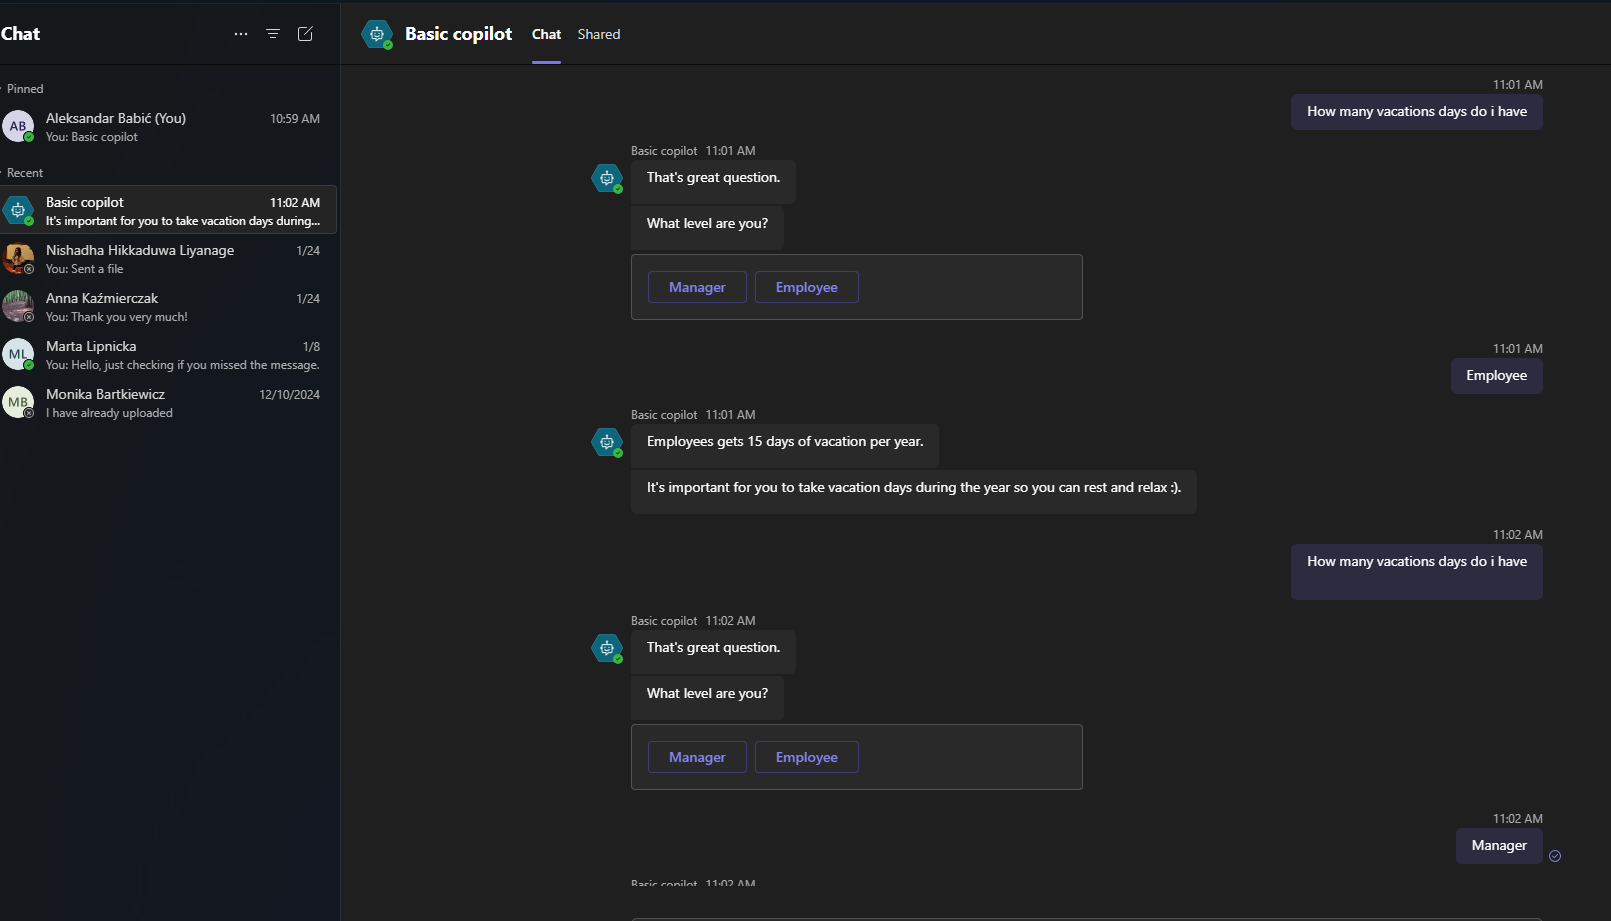
\includegraphics[width=0.8\textwidth]{./assets/Primjer_agenta_kreiranog_u_Copilot_Studiu.png} 
    \caption{Primjer copilota kreiranog u Microsoft Copilot Studiu}
    \label{fig:slika2}
\end{figure}

Osim toga isproban je i Bing Custom Search koji je vanjski servis koji se može koristiti za navođenje više izvora koji se koriste za odgovaranje na upite. Cilj je da se ne koristi cijeli
internet nego da se koristi taj skup podataka koji je naveden. Putem "custom configuration ID-a" može se povezati Custom Bing Search i Copilot Studio.
Naknadno isprobana je funkcionalnost Adaptive Cards Designer koji omogućava kreiranje vlastitih UI (eng. User Interface) elemenata koji se mogu koristiti unutar razgovora s korisnikom. 
Na sljedećoj slici može se vidjeti da je to JSON koji je potrebno importati u Copilot Studio. Na stranici \underline{https://adaptivecards.io/designer/} postoji veliki broj 
primjera koji su već kreirani i besplatni su za korištenje \cite{copilot2025}.

\begin{figure}[ht!]
    \centering
    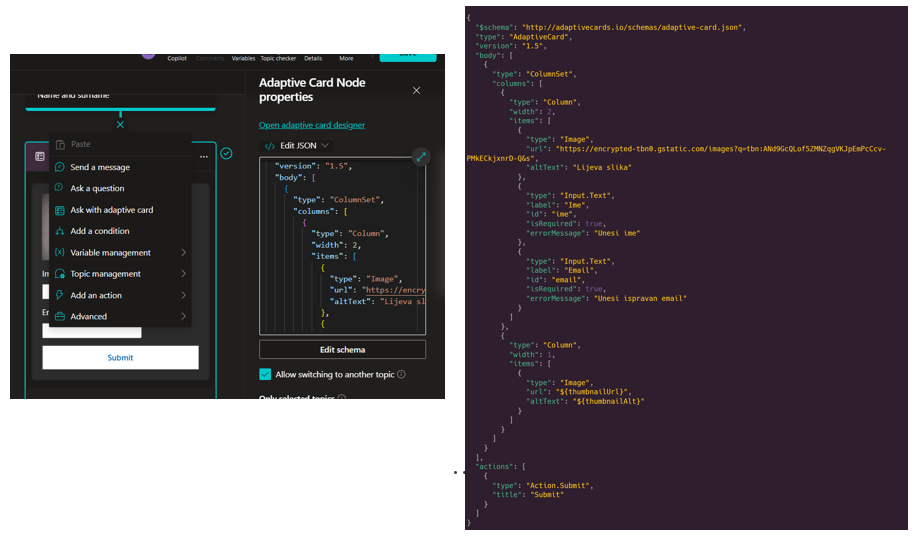
\includegraphics[width=1\textwidth]{./assets/Adaptive_cards.png} 
    \caption{Adaptive cards}
    \label{fig:slika3}
\end{figure}

Od drugih stvari koje još postoje u Copilot Studiju:
\begin{itemize}
\item Dvije vrste kreiranje entiteta (Copilot sadrži veliki broj entiteta koji se mogu koristiti ali se mogu kreirati i vlastiti (Closed List i Regular Expression)),
\item Message variation koji omogućava postojanje nekoliko verzija incijalnih poruka koje se pojavljuju kada se copilot pokrene. 
\end{itemize}

\subsection{Agent}

AI agenti predstavljaju vrhunac automatizacije i autonomije jer su sposobni samostalno donositi odluke i poduzimati radnje bez stalnog ljudskog vodstva. Dizajnirani su za složena okruženja a 
također se dinamički prilagođavaju kako bi postigli definirane ciljeve. Djeluju samostalno kako bi analizirali podatke i odredili prioritetne zadatke. Prate sustave i okruženja, predviđaju i rješavaju 
potencijalne probleme prije nego što eskaliraju. Pri radu s složenijim problemima, identificiraju optimalnija rješenja. Bankarski agenti zamrzavaju kompromitirane račune kada se otkrije neovlašteni pristup s visokorizične lokacije.
Na primjer, prate stanje servera, otkrivaju anomalije, identificiraju kašnjenje pošiljka i proaktivno obavještavaju kupca nudeći naknadu ili alternative i poduzimaju korektivne mjere bez ljudske intervencije \cite{exomindset2025difference}.

\subsubsection{ChatGPT Operator}
ChatGPT Operator je agent koji može ići na web kako bi obavljao zadatke umjesto korisnika. Može pregledavati web stranicu i komunicirati s njom tipkanjem, klikanjem i pomicanjem.
Pojavio se je u siječnju 2025. godine i trenutno je još u fazi razvoja gdje se nastoji poboljšat rješenje na temelju povratnih informacija korisnika. Od Operatora se može zatražiti da obavi
širok raspon repetitivnih zadataka u pregledniku, kao što je ispunjavanje formi, naručivanje proizvoda, pa čak i stvaranje memeova. Operator je dostupan unutar PRO verzije na području SAD-a i pokreće se
na temelju modela CUA (eng. Computer-Using Agent). CUA je obučen za interakciju s grafičkim korisničkim sučeljima (eng. Graphical User Interface) - gumbima, izbornicima i tekstualnim poljima koje ljudi vide na zaslonu.
Ako se dogodi da se Operator susretne s izazovima ili ako napravi pogreške, u tom slučaju vraća kontrolu korisniku, osiguravajući glatko i korisničko iskustvo \cite{openai2024operator}. 

U nastavku se navodi jedan primjer koji ChatGPT Operator obavlja \cite{rileybrown2025tiktok}:
\begin{enumerate}
    \item Upravlja preglednikom i obavlja radnje u ime korisnika.
    \item Analizira podatke na temelju YouTube veze.
    \item Generira PNG sliku analize.
    \item Ide na X.com, lokalno odabire sliku i prenosi je.
    \item Lajka i komentira sliku.
    \item Često traži potvrdu prije izvođenja radnji.
    \item Može se koristiti za pretraživanje weba, kupnju ulaznica ili rezervaciju restorana.
\end{enumerate}
\newpage

\subsection{Chatbot}

Chatbotovi su sustavi temeljeni na kreiranim pravilima koji su osmišljena za izvršavanje određenih zadataka putem unaprijed definirane interakcije. Iako posjeduju dosta ograničenja jako se dobro
i brzo snalaze u dosljednom rješavanju jednostavnih repetativnih zadataka. Djeluju na temelju stabla odlučivanja ili prepoznavanja ključnih riječi ograničavajući svoju interakciju na unaprijed 
postavljene scenarije. Koriste se za automatizaciju zadataka gdje se obrađuje veliki broj ponavljajućih upita poput rezervacija ili narudžbi. Njihova mana je da se ne mogu prilagoditi izvan
svog programiranja što ih čini neprikladnim za složenije zadatke \cite{exomindset2025difference}.

\subsubsection{Intercom}
Interkom je platforma za korisničku podršku koja olakšava komunikaciju između kupaca i tvrtki. Poboljšava interakciju s kupcima putem brojnih komunikacijskih kanala koji uključuju
chat uživo i automatizirano slanje poruka. Intercom je moguće integrirati s drugim alatima i platformama kao što su SalesForce, HubSpot, Zendesk i Slack.

Chatbotovi su posebno zanimljivi jer su to inteligentni sustavi koji možda najviše rade s kupcima i samim time mogu dosta utjecati na profit i vrijednost tvrtke. Na sljedećoj slici može
se vidjeti kako se pretpostavlja da će globalno tržište chatbotova do kraja 2027. godine vrijediti 455 milijuna dolara. Ova procijenjena brojka za 2027. godinu (455 milijuna USD) izračunata
je na temelju tržišne vrijednosti u 2018. godini \cite{connell2025chatbot}. 

\begin{figure}[ht!]
    \centering
    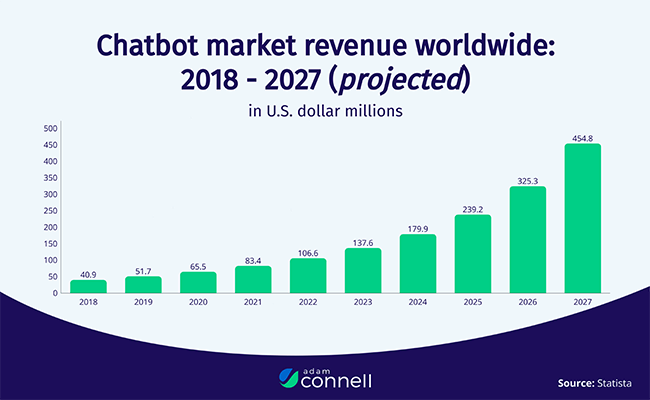
\includegraphics[width=0.65\textwidth]{./assets/chatbots.png} 
    \caption{Globalno tržište chatbotova; \href{https://adamconnell.me/wp-content/uploads/01-Chatbot-market-revenue.png}{Izvor}}
    \label{fig:slika3011}
\end{figure}

Također u sljedećem članku su doneseni sljedeći zaključci \cite{connell2025chatbot}:
\begin{itemize}
    \item Tvrtke mogu smanjiti troškove korisničke podrške za 30\,\% korištenjem chatbotova,
    \item Trećinu korisnika chatbotova čine tzv. „napredni korisnici”,
    \item Najveći uočeni nedostatak chatbotova jest njihova nemogućnost odgovaranja na složena i personalizirana pitanja,
    \item Čak 55\,\% ljudi radije bi koristilo chatbota nego čekalo dostupnost agenta uživo.
\end{itemize}

\newpage
\section{Inteligentni asistenti u obrazovnom sustavu}

Današnje obrazovanje se sve više oslanja na tehnologiju, a inteligentni asistenti postaju alat koji može poboljšati iskustvo učenja i poučavanja. Na primjer, svaki učenik može imati
personaliziranu pomoć, a učitelji imaju više vremena za fokusiranje na ono što je zaista važno. Takvi asistenti mogu prilagođavati materijale, odgovarati na pitanja, ocjenjivati domaće zadaće
čime se rasterećuje profesore. Jedna od najvećih prednosti koje donose inteligentni asistenti je personalizirano učenje. Umjesto univerzalnog pristupa, asistenti se mogu individualno 
posvetiti svakom učeniku/studentu. 

\subsection{Primjena inteligentnih asistenata u obrazovanju}

    \textbf{Automatizacija procesa ocjenjivanja} - ocjenjivanje pismenih zadataka, pružajući detaljne povratne informacije u roku od nekoliko minuta umjesto dana. 
    Osim što skraćuje vrijeme ocjenjivanja profesorima, učenici dobivaju brže povratne informacije o svom radu. Jedan od primjera je \href{https://www.gradescope.com/}{\underline{Gradescope}} kojeg je razvio Turnitin. 
    Kroz Gradescope moguće je ocjenjivati zadatke iz različitih predmeta, uključujući programiranje, fiziku, matematiku, kemiju, biologiju i ekonomiju. Također moguće je ocjenjivati
    programske projekte (u digitalnom obliku) i zadatke napisane na papiru. Neki od komentara profesora koji su koristili Gradescope su \cite{gradescope2025}:  
    \begin{itemize}
        \item "S Gradescopom je čast ocjenjivati. Prije što sam radio u rasponu od 2 do 3 sata sada odradim u 15 minuta" - Romulo Chumacero - University of Chile
        \item "Statistika mi stvarno pomaže da shvatim što sljedeći put mogu drugačije objasniti kako bih pomogla svojim učenicima da bolje uče" - Katie Johnson - Florida Gulf Coast University
        \item "Gradescope omogućuje da svaki dan svojoj grupi od 60 učenika dam kratki kviz i da ih sve ocijenim tijekom 30-minutne vožnje vlakom kući." -  Jesse Tov - Nortwestern University
    \end{itemize}

    \begin{figure}[ht!]
    \centering
    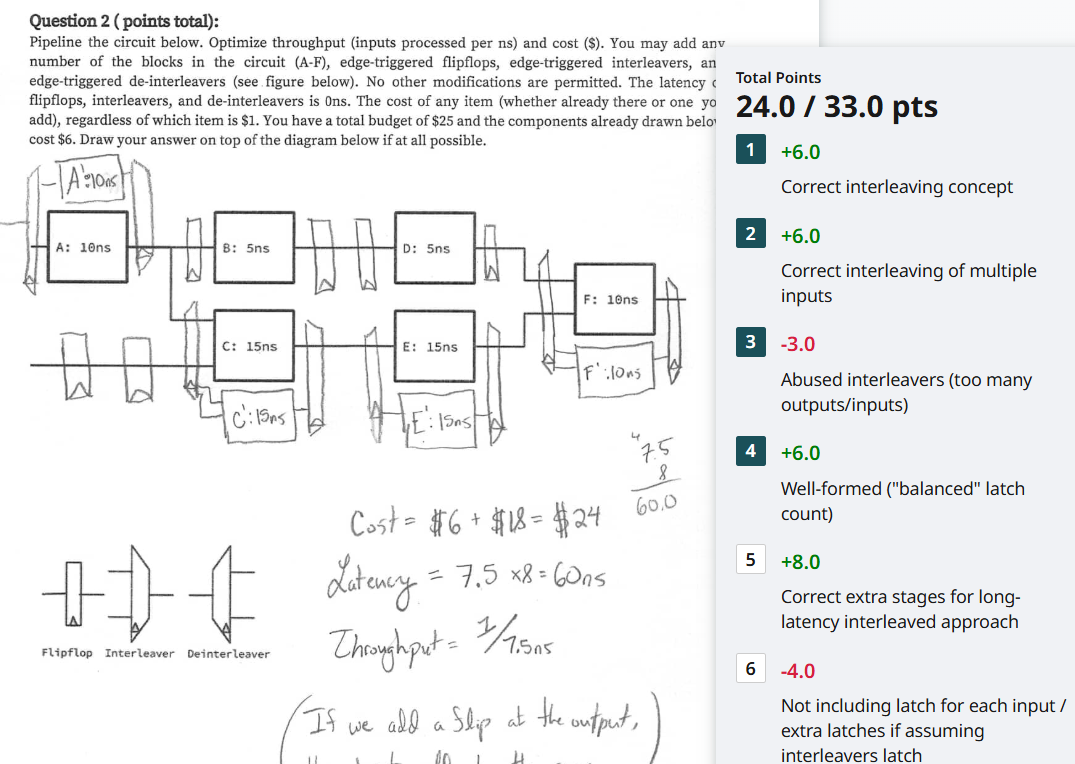
\includegraphics[width=0.8\textwidth]{./assets/Gradescope.png} 
    \caption{Ocjenjivanje zadatka - Gradescope \cite{gradescope2025}}
    \label{fig:slika7}
    \end{figure}

    \textbf{Smanjenje adminstrativnog opterećenja} - na primjer, sustavi pokretani umjetnom inteligencijom mogu pratiti prisutnost, upravljati zadacima pa čak i predviđati kojim
    studentima je potrebna dodatna pomoć. Takav pristup pomaže u otkrivanju problema prije nego što postane još veći problem. Jedan od zanimljivijih citata od Rose Luckin, profesorice dizajna
    usmjerenog na učenike na University College London, je: "Prava moć inteligentnih agenata u obrazovanju ne leži u zamjeni učitelja, već u pojačavanju njihovog utjecaja. Obavljanjem rutinskih
    zadataka, AI assistenti oslobađaju edukatore da se usredotoče na ljudske elemente poučavanja, inspiraciju, mentorstvo i njegovanje vještina kritičkog razmišljanja" \cite{weber2025smythos}. 
    
    
    \textbf{Prilagođavanje nastavnih materijala}   - analiziranje snaga, slabosti i načina učenja svakog učenika kako bi se stvorili prilagođeni materijali. Na primjer, ako postoji
    učenik koji se muči s razlomcima, asistent može pružiti dodatne resurse kako bi se poboljšalo njegovo razumijevanje \cite{weber2025smythos}.


\subsection{Izazovi inteligentnih asistenata u obrazovanju}

Jedan od najvećih izazova je pitanje privatnosti podataka. Obično sustavi zahtijevaju ogromne količine podataka o studentima da bi učinkovito funkcionirali, što ukazuje na opasnost od 
potencijalne zlouporabe tih podataka. Na primjer, studija Svučilišta u Michiganu iz 2020. godine otkrila je da 86 \,\% obrazovnih aplikacija umjetne inteligencije prikuplja osobne podatke od studenta,
a samo 42 \,\% ima jasne politike privatnosti \cite{weber2025smythos}.

Asistenti su dobri onoliko koliko su dobri podaci na kojima su obučeni. U obrazovnom sustavu, osiguranje kvalitete i relevantnosti tih podataka je od najveće važnosti.
Kako bi rješenje bilo zadovoljavajuće škole i programeri moraju surađivati kako bi stvorili sustave koji su ne samo učinkoviti, već i etični i sigurni \cite{weber2025smythos}.

Implementacija inteligentnih asistenata zahtijeva značajnu tehnološku infrastrukturu. Mnoge škole, posebno u ruralnim područjima, nemaju potreban hardver, brzi internet ili softver za podršku ovim sustavima.
Izvješće za obrazovanje iz 2022. godine kaže da gotovo 17 milijuna učenika u SAD-u još uvijek nema pristup internetu kod kuće \cite{weber2025smythos}.

Unatoč tim izazovima, integracija inteligentnih asistenata u obrazovni sustav donosi brojne prednosti. Sustavi pokretani umjetnom inteligencijom mogu automatizirati dugotrajne administrativne
zadatke, oslobađajući učitelje da se usredotoče na ono što najbolje rade: inspiriranje i poučavanje učenika. Osim toga, AI asistenti mogu pružiti personalizirano učenje, povećanu produktivnost
i učinkovitost, te poboljšano korisničko iskustvo \cite{weber2025smythos}.

Kroz sljedeće poglavlje je prikazano kako funkcioniraju inteligentni asistenti temeljeni na RAG (eng. Retrieval-Augmented generation) tehnologiji.
\newpage
\chapter{Retrieval Augmented Generation metoda}

U ovom poglavlju obrađena je RAG (eng. Retrieval Augmented Generation) metoda, koja predstavlja suvremeni pristup u području obrade prirodnog jezika i kombinira sposobnosti generativnih modela
s mehanizmima za dohvaćanje informacija iz vanjskih izvora. Poglavlje započinje pregledom povijesti a zatim slijedi teorijska osnova modela i njegova arhitektura
kroz faze dohvaćanja i generiranja. Nadalje je opisana primjena RAG-a, prednosti i izazovi te je zaključeno s pregledom dostupnih alata i biblioteka za implementaciju RAG sustava.

\section{Uvod u RAG}

RAG je proces optimizacije izlaza velikog jezičnog modela pri čemu se referencira na autoritativnu bazu znanja izvan izvora podataka za obuku 
prije generiranje odgovora. Veliki jezični modeli (eng. Large Language Models - LLM) obučavaju se na ogromnim količinama podataka i koriste milijarde parametara za 
generiranje izlaza za zadatke poput odgovaranja pitanja, prevođenja jezika i dovršavanja rečenica. Ideja RAG-a je da proširi već moćne mogućnosti 
LLM-ova na određene specifične domene, a sve to bez potrebe za ponovnom obukom modela. Takav pristup poboljšava LLM-ove u smislu točnosti, 
korisnosti i relevantnosti \cite{awsRAG2025}.

Model velikog jezika može se zamisliti kao entuzijastičnog zaposlenika koji odbija biti informiran o aktualnim događajima, ali uvijek odgovara
na pitanja s visokim samopouzdanjem. Nažalost, takav stav može negativno utjecati na povjerenje korisnika i nije nešto što bi trebalo postojati
kod AI sustava. Iz takvih razloga RAG tehnologija preusmjerava LLM kako bi dohvatio relevantne informacije iz unaprijed definiranih izvora znanja \cite{awsRAG2025}.

Bez RAG-a, LLM uzima korisnički unos i stvara odgovor na temelju informacija na kojima je obučen. S RAG-om se uvodi komponenta za pronalaženje 
informacija koja koristi korisnički unos kako bi prvo privukla informacije iz novog izvora podataka. Nakon toga LLM kombinira novo znanje i svoje 
podatke za stvaranje boljih odgovora \cite{awsRAG2025}.

Primjerice, ako se postavi pitanje: "Koji planet u Sunčevom sustavu ima najviše satelita?", osoba može odgovoriti: "Odlično pitanje! Kao dijete sam volio astronomiju i pročitao sam članak o tome
- mislim da je to Jupiter s 88 satelita." Međutim, takav odgovor ima nekoliko problema: osoba ne navodi konkretan izvor, iako nastupa s visokim samopouzdanjem ("ja to znam, pročitao sam")
te informacija može bit zastarjela jer se temelji na sjećanju iz prošlosti \cite{ibm2023rag}.

Kada bi osoba rekla: "Idem prvo na NASA-inu stranicu i tamo ću potražit tu informaciju", tada bi traženje odgovora bilo temeljeno na provjerenom i ažurnom izvoru.
Nasuprot tome, LLM-ovi, poput GPT-a, često odgovaraju vrlo samouvjereno, primjerice: "Na temelju podataka na kojima sam treniran, odgovor je Jupiter."
Iako zvuči uvjerljivo, takav odgovor može biti netočan, a korisnik često nije svjestan ograničenja modela ni datuma do kojeg je model treniran. U ovom slučaju, točan odgovor 
zapravo može biti Saturn, koji trenutno ima 114 poznatih prirodnih satelita. Rješenje za ovaj problem je korištenje spremišta znanja (eng. content store) koje može sadržavati izvore poput
internetskih stranica, PDF dokumenta ili baza podataka. LLM tada prvo pristupa tom vanjskom spremištu informacija, pretražuje ga, identificira relevantne sadržaje i tek tada generira
odgovor na temelju tih aktualnih podataka. U RAG sustavu prompt se najčešće sastoji od tri dijela: instrukcija (što model treba učiniti), korisnikovog upita (pitanje ili zahtjeva) i informacija 
koje su dohvaćene iz spremišta znanja \cite{ibm2023rag}.

Još jedan primjer je situacija u kojoj Alice želi saznati koliko dana porodiljnog dopusta može dobiti. AI sustav koji ne koristi RAG odgovara veselo i netočno ”Uzmi koliko želiš”.
Politike o porodiljnom dopustu su složene i razlikuju se ovisno o državi u kojoj se boravi. U ovom slučaju, veliki jezični model (LLM), umjesto da prizna ograničenje u znanju odgovarajući
"Žao mi je, ne znam", generirao je frazu iz svog skupa za treniranje koristeći korisnički orijentiran, ali neutemeljen jezik \cite{ibmRAG}.

\subsection{Povijest i razvoj}

Korijeni RAG-a mogu se pratiti od 1950-ih i 1960-ih kada su se koristili sustavi za pronalaženje informacija. Istraživači Hans Peter Luhn i Gerald Salton postavili su temelje za modele
vektorskog prostora omogućujući računalima da pronađu dokumente koji su relevantni za korisničke upite. Obrada prirodnog jezika značajnije je napredovala u 1980-ima i 1990-ima putem
statističkih jezičnih modela, poput n-gram modela \cite{custom_ai_studio2025}. 

Integracija pretraživanja i generiranja pojavila se u 2000-ima s razvojem sustava poput IBM Watsona, koji je koristio metodu pretraživanja za prikupljanje informacija i statističke modele 
za generiranje odgovora. Razvoj neuronskih mreža u 2010-ima dodatno je ubrzao ovu integraciju. Transformatori omogućuju značajan napredak u modeliranju jezika, dok tehnike gustog pretraživanja,
poput pretraživanja temeljenog na ugrađivanju, dodatno poboljšavaju točnost pretraživanja \cite{custom_ai_studio2025}. 

RAG se pojavljuje u radu "Retrieval-Augmented Generation for Knowledge-Intensive NLP Tasks" 2020. godine, gdje su autori predložili sustav u kojem vanjski model dohvaća relevantne
dokumente kao odgovor na upit, a generativni model uvjetovan tim dohvaćenim znanjem daje odgovor. U radu su autori koristili bi-enkoder za pretraživanje, temeljen na pretraživanju gustih prolaza
(eng. Dense Passage Retrieval) i T5 transformator kao generativni model, pokazajući izvanredne performanse na testovima koji zahtijevaju puno znanja. 
Ovaj pristup rješava ključne izazove s kojima se suočavaju modeli velikih jezika, poput halucinacija i zastarijelog znanja \cite{custom_ai_studio2025}. 

Objavljivanje RAG okvira potaknulo je nagli rast istraživanja, gdje je napravljeno nekoliko napredaka koja su se nadovezala na izvorni koncept \cite{custom_ai_studio2025}:

\begin{itemize}
    \item \textbf{Poboljšani modeli pretraživanja} - modeli neuronskog pretraživanja poput ColBERTa postaju standard u RAG sustavima,
    \item \textbf{Skalabilnost i učinkovitost} - kako bi se obradile ogromne količine podataka. Tehnike poput pretraživanja najbližeg susjeda (ANN) i destilacije modela pomogle su u optimizaciji performansi,
    \item \textbf{Primjene specifične za domenu} - do 2023. godine RAG sustavi su se prilagođavali specifičnim slučajevima upotrebe, kao što su pravne i medicinske domene, gdje su točnost i objašnjivost ključne stavke. Dodatno se je istraživalo fino podešavanje kako bi se dobio što precizniji odgovor, 
    \item \textbf{Multimodalni RAG} - proširivanje RAG-a kako bi uključio tekst, slike, zvuk i video. Proširivanje na područja poput obrazovanja i zabave, 
    \item \textbf{Prilagođeno učenje i petlje povratnih informacija}  - prilagodba prema korisnicima je ostvarena kroz razumijevanje njihovih povratnih informacija u stvarnom vremenu.
\end{itemize}

Kroz povijest RAG-a pokazuje se kako su se temeljna istraživanja u odvojenim područjima, poput pretraživanja i generiranja podataka, spojila kako bi se riješili izazovi u zadacima koji zahtijevaju puno znanja.
Također može se vidjeti važnost interdisciplinirane suradnje u području umjetne inteligencije, gdje se otkrića često javljaju kombiniranjem različitih metodologija \cite{custom_ai_studio2025}. 

\begin{figure}[h]
  \centering
  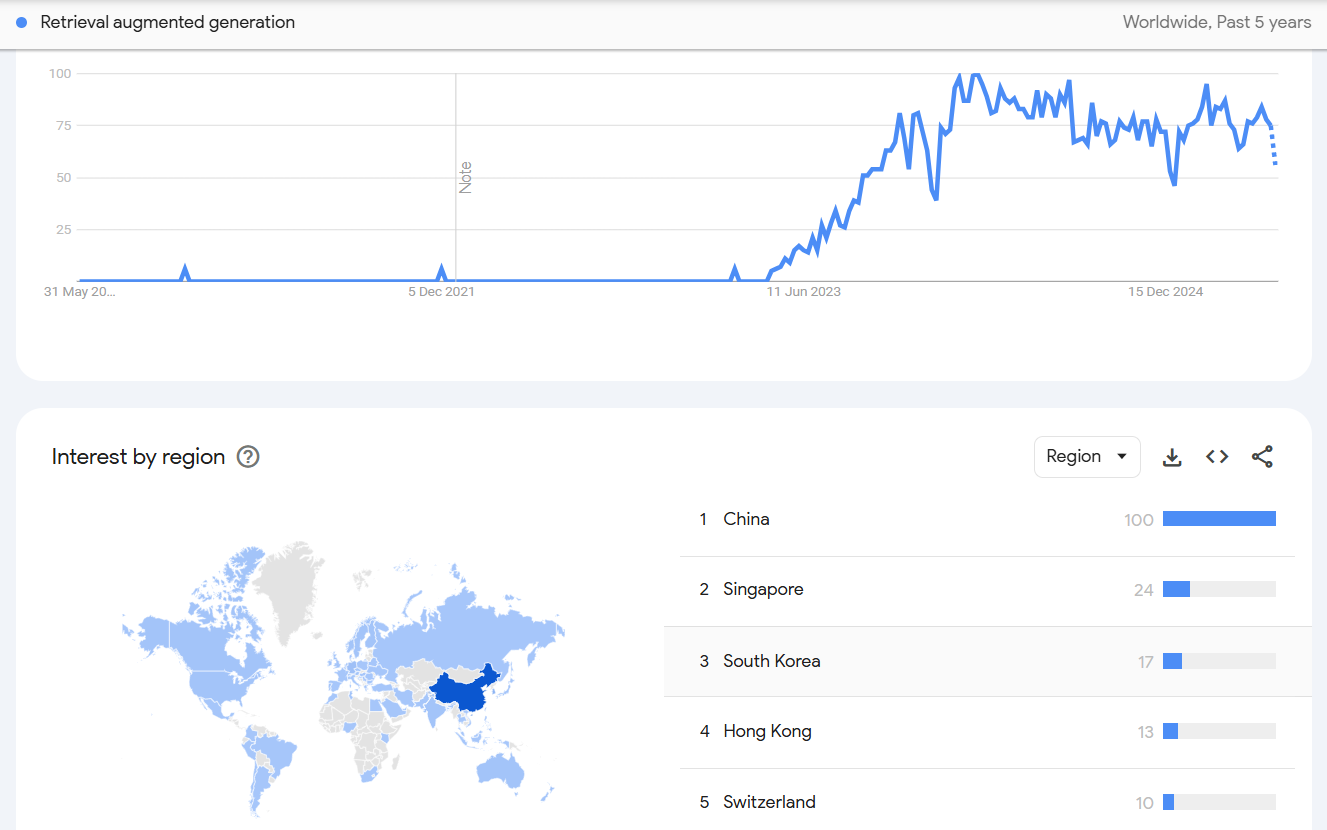
\includegraphics[width=1\textwidth]{./assets/PopularnostRaga.png}
  \caption{Popularnost RAG-a; \href{https://tinyurl.com/3cjn7n7k}{Izvor}}
  \label{fig:slika8}
\end{figure}

Važnost RAG-a povećala se posljednjih godina zbog pojave velikog broja aplikacija temeljenih na umjetnoj inteligenciji. Na slici \ref{fig:slika8}. se može vidjeti kako uzlazna putanja popularnosti RAG-a kreće od petog mjeseca 2023. godine.


\section{Arhitektura RAG modela}
RAG se sastoji od faze pronalaženja i faze generiranja sadržaja. U fazi pronalaženja algoritmi traže relevantne informacije za korisnikov upit dok se u fazi generiranja generira tekst 
kako bi se odgovorilo na korisnički upit. U okruženju otvorene domene te činjenice uglavnom dolaze iz indeksiranih dokumenata na internetu. U okruženju zatvorene domene obično se koristi 
uži skup izvora radi dodatne sigurnosti i pouzdanosti. Prije LLM-a, agenti su kroz razgovor pratili ručni tijek dijaloga. Pretpostavljali su namjeru klijenta, dohvaćali tražene informacije 
i dostavljali odgovor za određeni scenarij. Za jednostavne upite, ova ručna metoda stabla odlučivanja funkcionirala je sasvim dobro. Problem takvog pristupa je da se je gubilo vrijeme na 
pisanje i predviđanje svakog pitanja koje bi korisnik mogao postaviti. U takvim slučajevima, ako tražena informacija nije definirana u dostupnim podacima, AI sustav neće bit u mogućnosti 
pružiti relevantan odgovor\cite{ibmRAG}. 

Generalno RAG arhitektura se može objasniti kroz sljedeće karakteristike \cite{awsRAG2025}:

\begin{enumerate}
    \item \textbf{Stvaranje vanjskih podataka} - novi podaci izvan orginalnog skupa podataka koji su se koristili za treniranje LLM-a se zovu 
    vanjski podaci (eng. external data). Oni dolaze iz više izvora podataka kao što su: API-ji ili baze podataka. Podaci mogu postojati u različitim formatima.
    Jedna od tehnika (eng. embeeding language models) pretvara podatke u numerički oblik i sprema ih u vektorsku bazu podataka 
    (kako bi generativni modeli umjetne inteligencije to mogli razumjeti).
    \item \textbf{Preuzimanje relevantnih informacija} - Korisnički upit pretvara se u vektorski prikaz i uspoređuje se s vektorskim bazama podataka.
    Na primjer, ako korisnik postavi pitanje chatbotu "Koliko dana godišnjeg odmora imam?", AI sustav će morati preuzeti dokumente o politici godišnjeg 
    odmora uz evidenciju prošlih odmora za pojedinog zaposlenika. Takvi dokumenti će biti vraćeni korisniku jer su relevantni za njegov upit.
    \item \textbf{Proširivanje LLM upita} - Zatim, RAG model proširuje korisnički upit dodavanjem relevantnih dohvaćenih podataka u kontekstu. 
    Prošireni upit omogućuje modelima velikih jezika generiranje točnih odgovora na korisničke upite.
    \item \textbf{Ažuriranje vanjskih podataka} - Vrlo je bitno održati ažurne informacije i to se može ostvariti automatiziranjem procesa u stvarnom vremenu ili periodičnoj obradi. 
\end{enumerate}

Današnji AI sustavi bazirani na LLM-ovima mogu dati korisnicima odgovore bez da ljudi pišu definirane skripte. Samim nadovezivanjem RAG-a na LLM-ove smanjuje se potreba za ponovnim obučavanjem 
modela na novim primjerima \cite{ibmRAG}. Upiti korisnika nisu uvijek jednostavni, mogu biti dvosmisleno formulirani, složeni ili mogu zahtijevati znanje koje model nema. U takvim uvjetima 
LLM-ovi su skloni izmišljanju stvari. Rod Lastra opisuje velike jezične model kao “Zamislite model kao pretjerano nestrpljivog mlađeg zaposlenika koji izbrblja odgovor prije nego što provjeri činjenice”
Lastra dodatno ističe važnost svjesnog upravljanja neizvjesnošću u odgovaranjum, navodeći: “Iskustvo nas uči da zastanemo i kažemo kada nešto ne znamo. LLM-ovi moraju biti eksplicitno obučeni da prepoznaju pitanja na koja ne mogu odgovoriti” \cite{ibmRAG}. 

Sljedeća slika objašnjava kako RAG funkcionira na konkretnom primjeru. Ulaz u RAG sustav mogu biti različite vrste dokumenta, poput PDF-ova ili CSV datoteka. Nakon toga čita se 
sadržaj dokumenta i dijeli se u manje dijelove (eng. chunks) koji se mogu lakše obraditi. Svaki od tih dijelova pretvara se u vektor koristeći model ugrađivanja (eng. embedding model)
koji pretvara tekstualne podatke u numerički oblik. Ti vektori se zatim pohranjuju u vektorsku bazu podataka koja omoguće brzi pretraživanje informacija. Nakon toga dolazi do korisničkog
upita koji se također pretvara u vektor. Taj vektor se uspoređuje s vektorima u bazi podataka kako bi se pronašle relevantne informacije. Nadalje se rangiraju rezultati i odabiru oni
najrelevantniji. Na kraju, LLM koristi te informacije za generiranje odgovora na korisnički upit.

\begin{figure}[ht!]
    \centering
    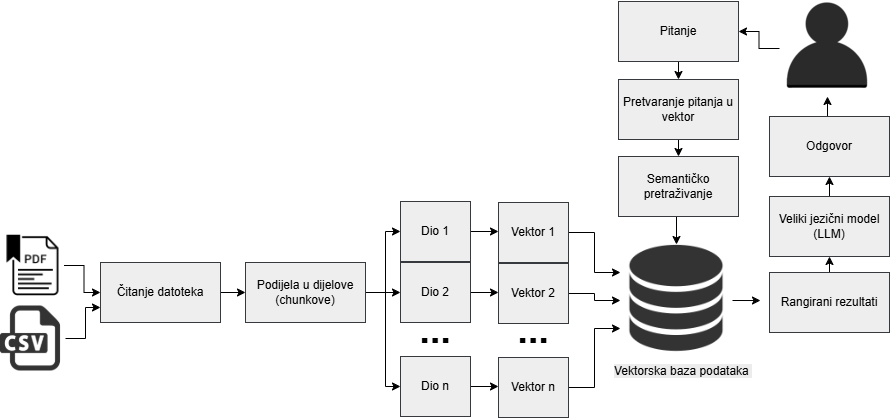
\includegraphics[width=0.8\textwidth]{./assets/rag_diagram.png} 
    \caption{Konceptualni tok korištenja RAG-a s LLM-ovima \cite{awsRAG2025}}
    \label{fig:slika1}
\end{figure}

 Jedna od zanimljivih stvari ovdje su vektorske baze podataka koje se mogu učinkovito indeksirati, pretraživati te je u njih jednostavno pohraniti veliku količinu informacija o čemu
 će se reći nešto detaljnije u jednom od sljedećih poglavlja.
 

\subsection{Faza dohvaćanja (Retriever)}

Retriver je komponenta koja je odgovorna za pronalaženje relevantnih dokumenata na temelju ulaznog upita. Retriver bilježi složenije semantičke odnose između upita i dokumenta, što dovodi do točnijih
rezultata dohvaćanja. Retriver može ugraditi dokumente i upite u visokodimenzionalni vektorski prostor, gdje udaljenost između vektora odgovara relevantnosti dokumenta za upit.
Dokumenti koji imaju veću "udaljenost" su manje relevantni za ulazni upit i time se mogu protumačiti kao nebitni. Retriver uzima ulazni upit, pretvara ga u vektor pomoću koder upita, a zatim
pronalazi najsličnije vektore dokumenta. Dokumenti povezani s tim vektorima se naknadno prosljeđuju generatoru. Broj dokumenta dohvaćenih u bilo kojem trenutku može se prilagoditi na temelju
specifičnih zahtjeva zadatka i obično za zadatke koji su kompleksniji može se pozvati opsežniji skup dokumenata.  Bitan aspekt kod retrivera je da se obrati pažnja na točnost dohvaćenih dokumenta
tijekom pronalaženja. Postavljanje praga za udaljenost nije isključivo tehnička odluka, već i poslovna odluka. Prag bi trebao biti usklađen s općim ciljevima, bilo da se radi o pružanju
sveobuhvatnog pregleda ili navođenju konkretnih detalja \cite{redis2025}. 

Korisnik postavlja pitanje ili šalje upit nakon čega retriver traži relevantne dokumente u unaprijed definiranom izvoru znanja (npr. Wikipedia, interni podaci tvrtke ili online članci).
Nakon toga se rangiraju dokumenti na temelju njihove relevantnosti za upit i za kraj se odabrani dokumenti prosljeđuju sljedećoj komponenti - generatoru - kako bi se pomoglo mu u generiranju odgovora.
Retriver je važan jer za razliku od tradicionalnih AI modela, koji se oslanjaju samo na unaprijed obučene podatke, može dohvatiti informacije u stvarnom vremenu. Također korištenje 
vanjskih izvora pomaže u smanjenju AI halucinacija i omogućuje modelu da se referira na pozadinsko znanje, što dovodi do smislenijih odgovora \cite{shaheryar2025}.

\subsubsection{BM25}
BM25 (eng. Best Matching 25) je popularni algoritam koji koristi pojam frenkvencijsko inverzne dokumentne frekvencije (eng. term frequency-inverse document frequency - TF-IDF) za rangiranje dokumenata na temelju relevantnosti.
BM25 izračunava ocjenu relevantnosti dokumenta na temelju učestalosti pojavljivanja upita u dokumentu. Iako je učinkovit za podudaranja
između ključnih riječi, BM25 može imati ograničenja u razumijevanju semantičkih odnosa. Unatoč tome BM25 se široko koristi zbog svoje jednostavnosti
i učinkovitosti. Često se koristi za jednostavnije upite temeljene na ključnim riječima, gdje je važno brzo dohvaćanje relevantnih informacija \cite{gupta2024rag}.

\subsubsection{Dense Passage Retrieval}
DPR (eng. Dense Passage Retrieval) je predstavljen 2020.godine i predstavlja moderniji pristup pretraživanja informacija. Koristi gusti
vektorski prostor u kojem su upiti i dokumenti kodirani u višedimenzionalne vektore. DPR koristi arhitekturu bi-enkodera, gdje su upit 
i dokument kodirani odvojeno, što omogućuje učinkovito pretraživanje najbližeg susjeda. Za razliku od BM25, DPR se ističe u pretraživanju
semantičkih odnosa između upita i dokumenta, što ga čini pogodnim za složenije upite koji zahtijevaju dublje razumijevanje konteksta. DPR može
pronaći dokumente koji su kontekstualno povezani s upitom, čak i ako ne sadrže točne ključne riječi \cite{gupta2024rag}.

\subsubsection{REALM}
REALM (eng. Retrieval-Augmented Language Model) je model koji integira pronalaženje informacija i generiranje teksta u jednom sustavu.
Ključna inovacija REALM-a je da uči pronalaziti dokumente koji poboljšavaju performanse modela na određenim zadacima kao što je npr.
sažimanje teksta. Tijekom treninga REALM ažurira retriever i generativni model zajedno, osiguravajući da je proces pronalaženja optimiziran
za zadatak generiranja. REALM je treniran kako bi prepoznao dokumente koji nisu relevatni za upit, ali su korisni za generiranje odgovora.
U literaturi se često spominje da REALM nadmašuje BM25 i DPR u zadacima koji zahtijevaju kombinaciju pronalaženja i generiranja informacija \cite{gupta2024rag}.


%\url{https://redis.io/glossary/retrieval-augmented-generation/}

%\url{https://dev.to/shaheryaryousaf/understanding-the-key-components-of-rag-retriever-and-generator-1a1j}

%\url{https://denser.ai/blog/retriever-for-rag/}

\subsection{Faza generiranja (Generator)}

Generator je komponenta koja koristi dohvaćene dokumente i izvorni upit kako bi generirala odgovor. To je obično veliki model transformatora kao što je GPT3.5, GPT4, Llama2, Falcpm, PaLM i BERT.
Dohvaćeni dokumenti i ulazni upit ulančavaju se i unose u generator, koji zatim koristi kombinirani ulaz za generiranje odgovora pri čemu dohvaćeni dokumenti pružaju dodatni kontekst i informacije 
koje pomažu generatoru da bude informiraniji i precizniji u svojim odgovorima \cite{redis2025}. 

Generator je važan jer pretvara neobrađene podatke u konherentan i strukturiran tekst i osigurava da odgovori zvuče prirodno i privlačno. Također, spaja unaprijed obučeno znanje o umjetnoj inteligenciji
s dohvaćenim informacijama u stvarnom vremenu za najbolji mogući odgovor \cite{shaheryar2025}. 

\subsubsection{T5}
T5 (eng. Text-to-Text Transfer Transformer) je jedan od najčešće korištenih modela za zadatke generiranja u RAG sustavima. T5 je svestran model koji pretvara sve zadatke u tekstualni format, što ga čini pogodnim za širok spektar aplikacija.
Može se koristiti za odgovaranje na pitanja, sažimanje ili generiranje dijaloga. Kroz praksu se pokazalo da RAG modeli temeljeni na T5 nadmašuju
tradicionalne generativne model poput GPT-3 i BART-a u raznim zadacima kaš što su odgovaranje na pitanja ili sažimanje teksta \cite{gupta2024rag}.

\subsubsection{BART}
BART (eng. Bidirectional and Auto-Regressive Transformers) je model koji je prikladan za zadatke koji uključuju generiranje teksta 
iz nečistih ili neuređenih podataka. Za enkoder BART koristi dvosmjerni pristup, što znači da može razumijeti kontekst cijelog ulaza,
dok dekoder generira tekst na temelju tog konteksta. BART može rekonstruirati oštećene tekstove, što ga čini korisnim za zadatke poput
izvlačenja informacija iz nepotpunih ili neurednih podataka \cite{gupta2024rag}. 


\section{Primjena RAG modela}

Kroz ovo poglavlje istražena je primjena RAG-a. Na početku istaknut je jedan primjer koji je podijelio Siddharth Asthana u jednom od svojih
članaka na Linkedlnu. U članku se govori o tome kako je velika bolnička mreža integrirala RAG u svoj sustav podrške kako bi donijela bolje odluke.
Sustav se povezao s elektroničkim zdravstvenim kartonima i višestrukim medicinskim bazama podataka, što je dovelo do \cite{siddharth2025rag}:
\begin{itemize}
    \item Smanjenja pogrešnih dijagnoza za složene slučajeve za 30 \,\%,
    \item Smanjenje vremena koje su liječnici proveli pregledavajući literaturu za 25 \,\%,
    \item Povećanje ranog otkrivanja rijetkih bolesti za 40 \,\%.
\end{itemize}

U nastavku je navedno nekoliko domena u kojoj se RAG može primjenjivati \cite{nishtha2025rag}:

\begin{itemize}
    \item \textbf{Sustavi za korisničku podršku} - kupac postavlja pitanje, chatbot dohvaća relevantne informacije iz izvora kao što su baze znanja,
    često postavljena pitanja ili zapisi kupaca i pritom koristi generativni model za izradu personaliziranog odgovora na temelju dohvaćenih podataka.
    \item \textbf{Sažimanje i pretraživanje dokumenta} - korištenje naprednih tehnika dohvaćanja informacija kako bi se poboljšale mogućnosti velikih LLM-ova.
    Na primjer, Google-ov Vertex AI Search koristi prvo algortime poput ANN kako bi brzo prikupio rezultate i zatim primjenjuje modele dubokog učenja za ponovo 
    rangiranje kako bi se osiguralo da su najrelevatniji dokumenti prioritetni.
    \item \textbf{Medicinska dijagnostika i istraživanje} - korištenje ogromnih baza podataka medicinskog znanja, elektroničkih zdravstvenih kartona, kliničkih 
    smjernica i medicinske literature kako bi se podržalo zdravstvene djelatnike u postavljanju točnih dijagnoza i dobro informiranih odluka o liječenju. 
    Jedan od primjera je IBM Watson koji analizira podatke o pacijentima s opsežnom medicinskom literaturom i time pomaže liječnicima u dijagnosticiranju
    složenijih slučajeva. IBM Watson Health se također koristi za dijagnostiku raka i shodno tome predlaže preporuke lječenja.
    \item \textbf{Personalizirani sustavi učenja i podučavanja} - jedan od primjera je RAMO (eng. Retrieval Augmented Generation for MOOCs) koji se bavi problemom hladnog starta u preporukama tečajeva
    korištenjem LLM-ova za generiranje personaliziranih prijedloga tečajeva. RAMO pomaže u razumijevanju preferencija i ciljeva osobe, nudeći relevantnije mogućnosti tečaja.
    Na primjer, sveučilišta su počela uvoditi sustave podučavanja vođene RAG-om kako bi pomogli studentima u učinkovitijem snalaženju u materijalima, potičući dublje razumijevanje i bolje akademske rezultate.
    \item \textbf{Otkrivanje prijevara i procjena rizika} - sposobnost RAG-a da pristupi podacima u stvarnom vremenu i uključi ih tijekom postupka donošenja odluka.
    Financijske tvrtke poput JPMorgan Chasea koriste sustave za otkrivanje prijevara koje su vođene umjetnom inteligencijom. Takvi sustavi kontinuirano dohvaćaju i analiziraju podatke
    u stvarnom vremenu iz različitih izvora kako bi se pratile transakcije i time otkrile potencijalne prijevare. 
    \item \textbf{Preporuke proizvoda za e-trgovinu} - za razliku od tradiocionalnih sustava preporuka, RAG se dinamički prilagođava specifičnim potrebama kupca u stvarnom vremenu čime
    preporuke postaju relevantnije i točnije što rezultira povećanom prodajom.
    \item \textbf{Upravljanje znanjem u poduzeću} - posebno korisno kod velikih tvrtki s opsežnom dokumentacijom i izvorima podataka. 
\end{itemize}

\subsection{Ključne prednosti RAG sustava}
U nastavku, kroz tablicu su prikazane ključne prednosti RAG sustava, koje objašnjavaju zašto je ova tehnologija sve češći odabir u izradi modernih AI rješenja. Navedene karakteristike
posebno dolaze do izražaja u izradi inteligentnih asistentata koji trebaju pružati točne, relevantne i ažurirane informacije. 

\begin{table}[ht!]
    \centering
    \caption{Prednosti RAG-a \cite{awsRAG2025}}
    \begin{tabular}{|>{\centering\arraybackslash}m{5cm}|>{\raggedright\arraybackslash}m{10cm}|}
      \hline
      \textbf{Prednost} & \textbf{Opis} \\
      \hline
      Isplativa implementacija & Razvoj AI sustava započinje korištenjem temeljnog modela (eng. Foundation models). Temeljni modeli su obično dostupni putem API ključeva i obučeni su na širokom spektru generaliziranih i neoznačenih podataka. Računalni i financijski troškovi za treniranje takvih modela su jako visoki. \\
      \hline
      Trenutne informacije & Iako su izvorni podaci LLM-a relevantni za specifične potrebe, teško je održati relevantnost. RAG se može koristiti za izravno povezivanje LLM-a s feedovima društvenih medija, web stranicama s vijestima i samim time pružiti korisnicima najnovije informacije. \\
      \hline
      Povećano povjerenje korisnika & RAG omogućuje prikazivanje točnih informacija s navođenjem izvora ili citata. Korisnici također mogu pretraživati izvorne dokumente ako im je potrebno dodatno pojašnjenje. \\
      \hline
      Više kontrole za razvojne programere & Učinkovitije testiranje i poboljšavanje aplikacija. Kontroliranje i mijenjanje izvora informacija. Rješavanje i ispravljanje problema. \\
      \hline
    \end{tabular}
\end{table}
    

%\url{https://www.projectpro.io/article/rag-use-cases-and-applications/1059}

\section{Izazovi RAG pristupa}

LLM-ovi su ključna tehnologija umjetne inteligencije koja pokreće chatbotove. Priroda LLM-ova je takva da ponekad unose dozu nepredvidljivosti
u generiranje odgovora. Osim toga, podaci o LLM obuci su statični i imaju krajnji rok za znanje koje posjeduju. Negativne strane LLM-ova uključuju \cite{awsRAG2025}:

\begin{itemize}
    \item Iznošenje lažnih informacija kada na njih nema odgovora (nepoželjni efekti nazvani - halucinacijama), 
    \item Prikazivanje zastarjelih informacija kada korisnik očekuje aktualan odgovor,
    \item Izrada odgovora iz neautoriziranih izvora,
    \item Stvaranje netočnih odgovora zbog terminološke zbrke, različiti izvori obuke koriste istu terminologiju za opisivanje različite stvari.
\end{itemize}

Veliki jezični modeli mogu biti nekonzistentni što bi značilo da ponekad točno odgovore na pitanja, a drugi put nasumično pogađaju. Ako povremeno zvuče kao da nemaju pojma što govore, 
to je zato što ustvari nemaju pojma. LLM-ovi znaju kako se riječi statistički povezivaju, ali ne znaju značenje riječi kao ni cjelinu njih, poznatu kao rečenica. RAG također smanjuje potrebu 
korisnika da kontinuirano treniraju model na novim podacima i ažuriraju njegove parametre. Na taj način, RAG može smanjiti računalne i financijske troškove pokretanja chatbotova \cite{ibmRAG}.


Sljedeći izvor navodi sljedeće izazove kod RAG pristupa \cite{aimlabs2025rag}:
\begin{itemize}
    \item \textbf{Sadržaj koji nedostaje} - jedan od glavnih izazova je kada odgovor na upit korisnika nije prisutan u indeksiranim dokumentima. U takvim slučajevima sustav je sklon 
    generiranju obmanjujućih odgovora ili u nekim slučajevima ne prepoznaje da mu nedostaju potrebne informacije. Na primjer, idealno ponašanje
    u takvim slučajevima je najbolje priznati poput: "Žao mi je, ne znam", iako to većina sustava ne uspijeva, što dovodi do smanjenog povjerenja
    korisnika. Ovaj izazov se može umanjiti povremenim dodavanjem podataka, implementacijom povratnih informacija kroz pogreške kako bi se ukazalo na
    nedostatak informacija i uvođenje prestanka generiranja odgovora kada odgovor ne zadovoljava potrebe korisnika. 
    \item \textbf{Neoptimalno dohvaćanje i rangiranje} - u slučaju da odgovor postoji unutar indeksiranog skupa podataka, moglo bi se desiti da neće biti dovoljno visoko rangiran za dohvaćanje 
    npr. zbog neoptimalnih algoritama rangiranja. Algoritmi rangiranja koji se oslanjaju isključivo na rezultate sličnosti često zanemaruju kontekst
    i specifičnost. Ovaj izazov se može umanjiti poboljšavanjem mehanizama rangiranja uključivanjem metapodataka kao što su vrste dokumenata,
    autorstvo ili datum objavljivanja. Također može se umanjiti s eksperimentiranjem s jačim modelima rangiranja kako bi se vidjelo hoće li 
    se relevantniji dokumenti drugačije pozicionirati.
    \item \textbf{Proturiječne informacije} - proturiječne informacije mogu dovesti do toga da LLM generira zbunjujuće informacije (halucinacije). Na primjer, RAG sustav korisničke podrške
    dohvaća informacije zastarijele politike uz trenutne, uzrokovajući da LLM generira netočne ili zbunjuće odgovore. To se može riješiti dodatnim
    filtriranjem nebitnih i kontradiktornih informacija prije nego što dođu do LLM-a. Dodatno trebalo bi još provesti testiranja i fino podesiti
    upite kako bi se usmjerila pozornost LLM-a na najrelevantnije / najnovije informacije. 
    \item \textbf{Nepotpuni odgovori} - nepotpuni odgovori nastaju kada sustav ne uspije spojiti sve relevantne informacije. Na primjer, RAG sustav koji se bavi domenom prava i od njega
    se traži da sažme ključne točke tri različita slučaja, može se baviti samo jednim slučajem, izostavljajući kritične detalje iz ostala dva. 
    \item \textbf{Izazovi s performansama i skalabilnošću u pronalaženju} - takvi izazovi nastaju kada se sustav bori s učinkovitim rukovanjem skupova podataka velikih razmjera. Kako veličina skupa raste, latencija
    dohvaćanja se povećava zbog računalnih troškova u pretraživanju, rangiranju i dohvaćanju relevantnih dokumenata. 
\end{itemize}
\newpage


\subsection{Halucinacije}

AI halucinacije su izlazi iz modela koji značajno odstupaju od stvarnosti i često predstavljaju netočne ili izmišljene informacije kao istinite. Halucinacije nastaju kao rezultat inherentnih ograničenja
podataka za LLM obuku ili kada model ne uspije povezati namjeru ili kontekst upita s podacima potrebnim za generiranje smislenog odgovora. Iako je RAG osmišljen kako bi pomogao u smanjenju
AI halucinacija, RAG halucinacije se i dalje mogu pojavljivati. Na takve stvari treba pripaziti jer na primjer, pretplatnik mobilne mreže može dobiti netočan odgovor o svom prosječnom mjesečnom
računu od operaterovog RAG chatbota - jer podaci tvrtke možda uključuju račune koji nisu bili njegovi \cite{rag_hallucination2025}. 

AI halucinacije se mogu suzbiti kroz nekoliko pristupa \cite{rag_hallucination2025}:

\begin{itemize}
    \item \textbf{Fino podešavanje provjerom činjenica} - postoji sloj koji projerava činjenice prije nego što se generira odgovor. Nedosljednosti se označavaju, što potiče LLM da poboljša svoj 
    rezultat na temelju činjeničnih temelja. 
    \item \textbf{Navođenje izvora} - razumijevanje načina na koji generativna umjetna inteligencija dolazi do odgovora ključno je. Korisnicima se pokazuju izvori koji su korišteni za generiranje odgovora,
    čime je osigurana pouzdanost i transparentnost. 
    \item \textbf{Povezivanje modela s javnim podacima više kvalitete} - daje se prednost visokokvalitetnim, raznolikim i činjeničnim informacijama. Tehnike poput čišćenja podataka i filtriranja
    pristranosti mogu pomoći u smanjenju halucinacija.
    \item \textbf{Korištenje RAG-a za proširenje LLM-ova s privatnim organizacijskim podacima} - nadopunjavanje znanja s privatnim podacima organizacije može smanjiti rizik od izmišljenih odgovora.
\end{itemize}

RAG ne može u potpunosti eliminirati halucinacije i ograničen je kvalitetom podataka, kontekstualnom svijesti (možda se neće svaki put najbolje razumijet što korisnik želi - propuštanje poante prompta),
razmišljanjem (zdravi razum) i kreativnošću modela. 

%\url{https://www.k2view.com/blog/rag-hallucination/}


%\url{https://www.aimon.ai/posts/top_problems_with_rag_systems_and_ways_to_mitigate_them}


\newpage
\section{Dostupni alati i biblioteke}

U ovoj sekciji su navedeni neki od najpopularnijih alata i biblioteka koje se koriste za implementaciju RAG sustava. 
Izvršen je pregled i analiza svakog alata nakon čega je donesen zaključak koji od njih su korišteni u praktičnom dijelu rada.
Na sljedećoj slici može se vidjeti kratki sažetak alata i biblioteka koje se mogu koristiti za implementaciju RAG sustava.

\begin{figure}[h]
  \centering
  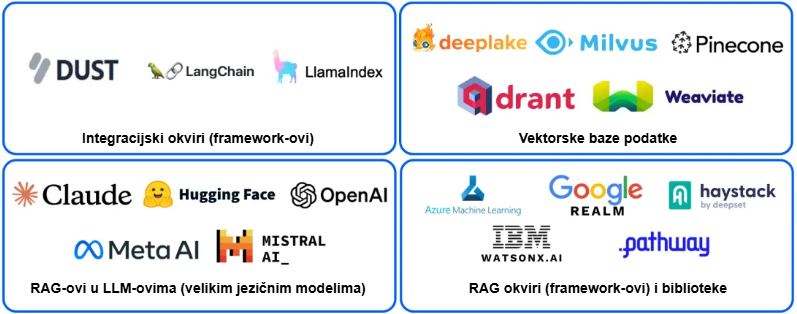
\includegraphics[width=0.7\textwidth]{./assets/sazetak_dostupni_alati.png}
  \caption{Sažetak dostupnih alata i biblioteka za razvoj RAG sustava; \href{https://tinyurl.com/eae6swbk}{Izvor}}
  \label{fig:slika9}
\end{figure}


%\url{https://lakefs.io/blog/rag-tools/}

%\url{https://www.firecrawl.dev/blog/best-open-source-rag-frameworks} - ovo je beskorisno

%\url{https://research.aimultiple.com/retrieval-augmented-generation/}

%\url{https://www.analyticsvidhya.com/blog/2024/05/rag-tools/}

%\subsection{Hugging Face Transformers + Datasets}

\subsection{Okviri (frameworkovi) za upravljanje RAG-om}
U nastavku su navedeni neki od najpopularnijih okvira koji se koriste za jednostavniju izgradnju, testiranje i održavanje sustava temeljenih
na RAG pristupu. Pružaju funkcionalnosti za povezivanje velikih jezičnih modela s vanjskim izvorima podataka kao što su baze podataka.
\subsubsection{Haystack}
Haystack je platforma za obradu prirodnog jezika otvorenog koda koja je specijalizirana za stvaranje RAG cjevovoda za sustave pretraživanja 
i odgovaranja na pitanja. Framework pruža komponente za dohvaćanje dokumenta, odgovaranje na pitanja i generiranje teksta, omogućujući korisnicima
da brzo i jednostavno izrade RAG aplikacije. Haystack se također povezuje s modelima kao što su BERT i RoBERTa, što poboljšava njegovu sposobnost 
rukovanja s težim upitima. Također Haystack ima API koji je prilagođen korisniku i korisničkom sučelju temeljenom na webu, omogućujući korisnicima
jednostavnu interakciju sa sustavom \cite{novogroder2025ragtools}.

Značajke koje Haystack nudi su \cite{novogroder2025ragtools}:
\begin{itemize}
    \item Podržavanje pozadinskih sustava za pohranu kao što su Elasticsearch, FAISS, SQL i InMemory,
    \item Pretraživanje na temelju ključnih riječi pomoću BM25,
    \item GenerativePipeline - kombiniranje retrivera i generatora (GPT - 3/4),
    \item TransformersReader - ekstrakcijska kontrola kvalitete koristeći Hugging Face modele,
    \item DensePassageRetriever - dohvaća gusto ugrađene vektore koristeći DPR (eng. Dense Passage Retrieval),
    \item EmbeddingRetriever - custom embeddings koristeći Hugging Face modele.
\end{itemize}

Vrlo lagano se može instalirati lokalno na Linux sustavu pomoću pip-a ili conde (pip install haystack-ai). Dokumentacija se nalazi na sljedećem linku - \url{https://docs.haystack.deepset.ai/docs/intro}. 

\subsubsection{LangChain}
Langchain je Python paket otvorenog koda koji pruža sveobuhvatanu osnovu za izgradnju aplikacija s velikim jezičnim modelima. Kombinira modularni i fleksibilni dizajn s sučeljem
visoke razine, što ga čini idealnim za razvoj RAG sustava. Također, LangChain omogućuje jednostavnu integraciju različitih izvora podataka, uključujući dokumente, baze podataka i API-je što pomaže u procesu
generiranja odgovora. Langchain nudi širok raspon funkcionalnosti i omogućuje korisnicima izmjenu i kombiniranje različitih komponenti kako bi odgovarale jedinstvenim zahtjevima aplikacije,
što olakšava stvaranje dinamičkih i prilagodljivih aplikacija \cite{novogroder2025ragtools}.

Značajke koje LangChain nudi su \cite{novogroder2025ragtools}:
\begin{itemize}
    \item Integracija s vektorskim bazama podataka kao što su Pinecone, Chroma i FAISS,
    \item Učitavanje i dohvaćanje podataka iz baza podataka, API-ja i lokalnih datoteka,
    \item Retriveri uključuju BM25, Chroma, FAISS i druge,
    \item Učitavanje PDF, teksta, web scrapinga i SQL/NoSQL baza podataka,
    \item Generiranje dinamičkih upita pomoću predloženih struktura.
\end{itemize}

Langchain se može instalirati lokalno na Linux sustavu koristeći pip (pip install -U langchain). Dokumentacija se nalazi na - \url{https://python.langchain.com/docs/introduction/} 


\subsubsection{LlamaIndex}
LlamaIndex je robusna biblioteka otvorenog koda koja se usredotočuje na učinkovito indeksiranje i dohvaćanje iz ogromnih skupova podataka. 
LlamaIndex koristi napredne tehnike kao što je pretraživanje vektorske sličnosti i hijerarhijsko indeksiranje kako bi se omogućilo brzo i 
točno dohvaćanje relevantnih informacija, poboljšavajući mogućnosti generativnih jezičnih modela. Lako se povezuje s uobičajenim 
velikim jezičnim modelima, omogućujući umetanje primljenih podataka u proces stvaranja i čineći ga učinkovitim alatom za poboljšanje performansi 
RAG sustava \cite{novogroder2025ragtools}.

\begin{itemize}
    \item Optimizirano je dohvaćanje s malom latencijom,
    \item Moguće je učitavanje različitih vrsta podataka kao što su: TXT, PDF, DOC, CSV, API-je, baze podataka i web scraping,
    \item Kombiniranje modela (OpenAI ili Hugging Face) s vektorskim bazama podataka,
    \item Sadrži više indeksa kao što su:
    \begin{itemize}
        \item \textbf{Indeks pohrane vektora} - se koristi za pohranu podataka kao vektora, što omogućuje brzo pretraživanje sličnosti kao što su sustavi za dohvaćanje dokumenata i sustavi preporuka,
        \item \textbf{Indeks popisa} - je jednostavan, sekvencijalan indeks za manje skupove podataka koji omogućuje brzo linearno pretraživanje,
        \item \textbf{Indeks stabla} - koristi hijerarhijsku struktru za izvođenje učinkovitih semantičkih pretraživanja čime je idealan za složene upite kod podataka gdje je jasna hijerarhija,
        \item \textbf{Indeks tablice ključnih riječi} - tablica mapiranja se koristi kako bi olakšala pretraživanje temeljeno na ključnim riječima.
    \end{itemize}
\end{itemize}

LlamaIndex je moguće instalirati pomoću naredbi pip install llama-index ili pip install llama-index-core. Dokumentacija se nalazi na sljedećem linku \url{https://docs.llamaindex.ai/en/stable/}.

\subsection{Vektorske baze podataka}
Tradicionalne baze podataka pohranjuju podatke u strukturiranom formatu (redci i stupci), dok vektorske baze podataka su optimizirane za rukovanje
visokodimenzionalnim vektorskim podacima i podržavaju operacije poput pretraživanja sličnosti i pretraživanja najbližih susjeda (k-NN). Umetanje
podataka se vrši kroz generiranje ugrađivanja (eng. embeddings) iz neobrađenih vrsta podataka (npr. teksta) i pohranjivanje tih ugrađivanja u vektorsku bazu podataka.
Vektorske baze podataka ključne su kako bi omogućile LLM-ovima da daju točnije i skalabilnije informacije. 
Osim toga, vektorske baze podataka omogućuju rad s bilo kojim drugim tipovima podataka, uključujući slike, videozapise i zvuk, čime se proširuju mogućnost RAG sustava.
Većina podataka koja se generira svakodnevno su nestrukturirani podaci, bilo to tekst, slike, videozapisi ili slično. 
Nestrukturiranim podacima nedostaje strogi format, što otežava upravljanje konvencionalnim bazama podataka i iako se ponekad čine beznačajnim,
oni sadrže vrijedne informacije koje imaju ogroman potencijal za umjetnu inteligenciju \cite{aquino2025vector}.

Tradicionalne baze podataka poput OLTP i OLAP odlično upravljaju s strukturiranim podacima, međutim kada se pojave podaci koji se ne mogu lako kategorizirati
poput sadržaja unutar PDF datoteka stvari počinju biti komplicirane. Takva baza ne može razumijeti što se nalazi u dokumentu, ne može ga kategorizirati ili pretraživati.
Vektorske baze podataka dobile su na značaju u posljednjih nekoliko godina zbog porasta strojnog učenja i dubokog učenja. Vektorska ugrađivanja
pretvaraju složene podatke (npr. slike ili tekst) u visokodimenzionalne vektore tako da su slične stavke bliže jedna drugoj u vektorskom prostoru \cite{aquino2025vector}.

Tradicionalne baze podataka su neučinkovite pri pretraživanju sličnosti u visokodimenzionalnim prostorima. Takav problem vrlo dobro rješavaju
vektorske baze podataka koje vrlo dobro indeksiraju i pretraživaju opsežne skupove podataka. Kako bi se proveo rad s vektorskim bazama podataka,
potrebno je koristiti vektor upita koji obuhvaća kriterije pretraživanja. Sljedeći korak je korištenje metrike sličnosti za određivanje blizine
između vektora upita i vektora u bazi podataka. To može uključivati metriku kao što su kosinusna sličnost, euklidska udaljenost ili Jaccardov indeks.
U prošlosti su samo velike tehnološke tvrtke koje su imale resurse za njihovo stvaranje i održavanje koristile vektorske baze podataka. S obzirom
na napredak tehnologije, pojavile su se mnoge vektorske baze podataka otvorenog koda koje su dostupne za korištenje i implementaciju u RAG sustavima.
Sljedeći grafikon prikazuje kada se koriste vektorske baze podataka u odnosu na tradicionalne baze podataka \cite{aquino2025vector}.

%\url{https://qdrant.tech/articles/what-is-a-vector-database/?q=what+is+wector+data}
%\url{https://research.aimultiple.com/retrieval-augmented-generation/}

\renewcommand{\arraystretch}{1.4}
\begin{table}[ht!]
\centering
\begin{tabular}{|>{\columncolor{blue!20}\bfseries}p{4cm}|p{3.5cm}|p{4cm}|p{4cm}|}
\hline
Karakteristika & OLTP baza podataka & OLAP baza podataka & Vektorska baza podataka \\
\hline
\rowcolor{blue!10}
Struktura podataka & Redci i stupci & Redci i stupci & Vektori \\
\hline
\rowcolor{blue!10}
Podaci & Strukturirani & Strukturirani / nestrukturirani & Nestrukturirani \\
\hline
\rowcolor{blue!10}
Metoda upita & SQL (Transakcije) & SQL (agregacije i analitički upiti) & Vektorsko pretraživanje na temelju sličnosti \\
\hline
\rowcolor{blue!10}
Fokus & Optimizirano za ažuriranje & Optimizirano za čitanje & Kontekst i semantika \\
\hline
\rowcolor{blue!10}
Slučajevi upotrebe & CRM, obrada narudžbi & Poslovna inteligencija, skladišta & RAG, otkrivanje anomalija \\
\hline
\end{tabular}
\caption{Usporedba OLTP, OLAP i vektorskih baza podataka \cite{aquino2025vector}}
\label{tab:usporedba_baza}
\end{table}

\begin{figure}[h]
  \centering
  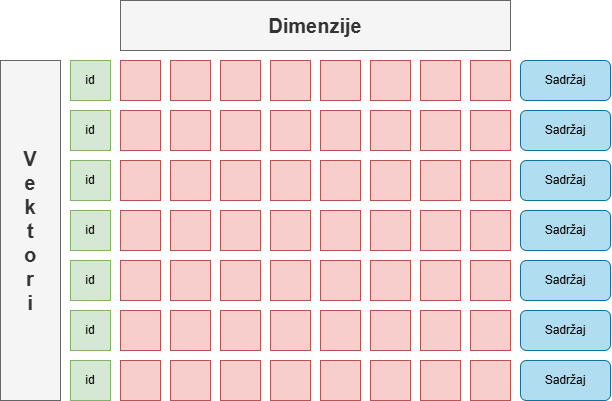
\includegraphics[width=0.6\textwidth]{./assets/payload.png}
  \caption{Vektorska baza - primjer; \href{https://tinyurl.com/469fzf35}{Izvor}}
  \label{fig:slika10}
\end{figure}

Prethodna slika prikazuje strukturu vektorske baze podataka. ID (zelena polja) predstavlja jedinstveni identifikator svakog vektora, 
primjerice doc01. Svaki redak u crvenoj matrici odgovara jednom vektoru, odnosno nizu brojeva koji predstavlja semantičko značenje 
određenog teksta. Plava polja označena kao payload sadrže dodatne informacije povezane s vektorom, poput originalnog teksta, metapodataka 
kao što su jezik i izvor, te putanje do dokumenta. Dimenzije vektora, prikazane u gornjem dijelu slike, određuju širinu svakog vektora, 
odnosno broj numeričkih vrijednosti koje ga čine.
\newpage

\subsubsection{FAISS}
FAISS (eng. Facebook AI Similarity Search) je robusna vektorska baza podataka koju je razvio Facevook-ov istraživačkim tim za umjetnu inteligenciju. Vrlo je učinkovita i brza, što je čini 
savršenim izborom za razvoj aplikacija u stvarnom vremenu specifičnih za industriju. Dostupno je nekoliko opcija indeksiranja, učinkovito grupira i izgrađena je 
na Pythonu i C++ jeziku. Jedne od poznatijih tvrtki koje koriste FAISS su Meta i Pinterest \cite{baghel2025vectors}. 

\subsubsection{Qdrant}
Qdrant je vektorska baza podataka koja je optimizirana za pretraživanje po sličnosti i omogućuje brzo i učinkovito pretraživanje velikih skupova podataka. Od dodatnih mogućnosti Qdrant nudi:
mogućnost preciznog pretraživanja, pametno pohranjivanje vektora, skalabilni dizajn prilagođen oblaku. Klijenti Qdranta su: Bosch, Johnson i Johnson i Discord \cite{baghel2025vectors}.
%\url{https://www.openxcell.com/blog/best-vector-databases/}

\subsubsection{Pinecone}
Pinecone je vektorska baza podataka u oblaku (eng. cloud-native) zatvorenog koda koja nudi upravljivost, skalabilnost i visoku učinkovitost. Jednostavnost, podrška za hibridne upite i uska integracija s strojim učenjem čine Pinecone 
popularnim izborom za RAG sustave. Značajke koje Pinecone nudi su: ažuriranje u stvarnom vremenu bez zastoja, visokodimenzionalno vektorsko pretraživanje u velikoj mjeri i integracija s Pythonom, Langchainom i drugima.
Neki od klijenta Pinecone su: Microsoft, Notion, Hubspot i Shopify.
Pinecone je vektorska baza podataka u oblaku koja je potpuno upravljana i ne zahtijeva nikako odražavanje infrastrukture \cite{baghel2025vectors}. 

\subsection{Veliki jezični modeli}
Veliki jezični model je napredni AI model koji može razumijeti i generirati ljudski jezik. U srži LLM-ova je strojno učenje, koje je podskup umjetne inteligencije i omogućuje 
sustavima učenje iz podataka i poboljšanje tijekom vremena bez eksplicitnog programiranja. Također koristi se duboko učenje kako bi se analizirala ogromna količina podataka. 
Neuronske mreže su jedna od opcija kod kojih se obučava model na velikim skupovima podataka kako bi se prepoznali odnosi između riječi i fraza.
LLM-ovi se mogu kategorizirati na mnogo načina no najčešći način kategorizacije je prema njihovoj arhitekturi i funkcionalnosti \cite{vermeir2025llm}:
\begin{itemize}
    \item Generativni modeli - osmišljeni za stvaranje visokokvalitetnog teksta nalik ljudskom u raznim formatima (GPT-4),
    \item Modeli enkodera-dekodera - specijalizirani za zadatke poput strojnog prevođenja i sažimanje teksta (primjer T5),
    \item Modeli samo s enkoderom - fokusirani na razumijevanje značenja teksta (primjer BERT),
    \item Multimodalni LLM-ovi - obrađivanje i generiranje više vrsta podataka, uključujući tekst, slike i zvuk. Koriste se zadatke poput 
    opisivanja slika, analize videa i multimodalnog pretraživanja kako bi se stvorila bogatija interakcija između različitih oblika
    podataka.
\end{itemize}

Na sljedećoj slici se može vidjeti kako je model OpenAI o1 predstavnik u riješavanju matematičkih modela za 2024. godinu.
\begin{figure}[h]
  \centering
  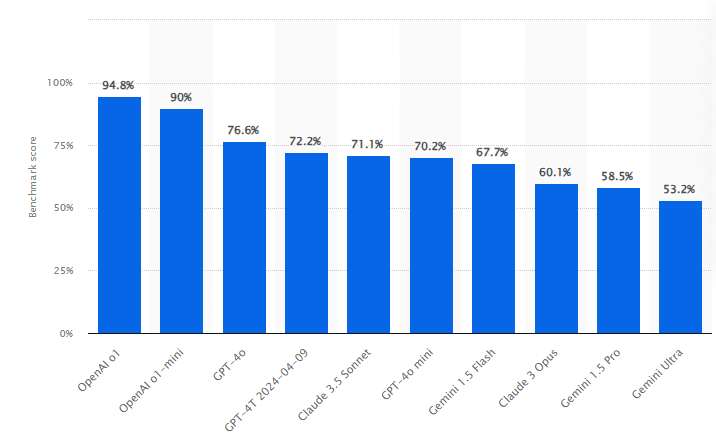
\includegraphics[width=0.6\textwidth]{./assets/Statista.png}
  \caption{Popularnost LLM-ova u rješavanju matematičkih problema za 2024 godinu; \href{https://www.statista.com/statistics/1458141/leading-math-llm-tools/}{Izvor}}
  \label{fig:slika310}
\end{figure}


%\url{https://mehmetozkaya.medium.com/llm-providers-openai-meta-ai-anthropic-hugging-face-microsoft-google-and-mistral-ai-46ad8c027f6b}

\subsubsection{OpenAI}
OpenAI je jedan od začetnika i najpoznatijih pružatelja usluga u području umjetne inteligencije. Poznat je po razvoju GPT modela, uključujući GPT-3 i GPT-4, kao i Codexa za generiranje koda.
Od dodatnih mogućnosti generira tekst, razumije jezik, pomaže pri kodiranju i može se koristiti za razvoj AI sustava i drugih aplikacija. Dostupan je putem OpenAI API-ja i putem Microsoftove usluge
Azure OpenAI \cite{ozkaya2025llm}.

\subsubsection{Hugging Face}
Hugging Face je platforma koja nudi širok spektar modela otvorenog koda a poznat je po svojoj biblioteci Transformers i Model Hub-u. Hugging Face nudi različite modela poput BERT-a, GPT-2 i T5-a koji se mogu koristiti za različite zadatke.
Transformers biblioteka koja omogućuje jednostavno korištenje i integraciju najsuvremenijih modela dubokog učenja. ModelHub je platforma na kojoj programeri i istraživači mogu prenositi, dijeliti i surađivati na modelima. Također Hugging 
Face potiče okruženje u kojem se dijeli znanje i resursi čime se ubrzava razvoj i potiče se na inovacije u području umjetne inteligencije \cite{ozkaya2025llm}.

%\subsubsection{Anthropic}
%Anthropic je tvrtka koja se fokusira na razvoj sigurnosnih i etičkih AI modela koji se ponašaju u skladu s ljudskim vrijednostima. Poznata je po seriji Claude modela \cite{ozkaya2025llm}. 
Zaključak je da su svi navedeni alati i biblioteke korisni za implemetaciju RAG sustava, ali za potrebe ovog rada korištena je kombinacija
Langchaina, ChatGPT (OpenAI) modela i FAISS vektorske baze podataka. 


\chapter{Korištene tehnologije i alati}
Za realizaciju praktičnog dijela korišteno je nekoliko tehnologija koje su omogućile razvoj web stranice i inteligentnog asistenta. 
Odabir tehnologija temelji se na njihovoj popularnosti, pouzdanosti i sposobnosti da zadovolje zahtjeve ovog rada. U nastavku su detaljnije
opisani korišteni alati i tehnologije.

\section{React}

Svijet danas ne funkcionira bez mobilnih i web aplikacija. Sve se orijentira prema digitalizaciji, od rezerviranja hrane do naručivanja vožnje u taksiju. Vrlo je bitno napraviti vizualno
primamljivu aplikaciju a React je upravo jedna od popularnijih frontend biblioteka koja to omogućava. React je temeljen na JavaScriptu i široko se koristi u web razvoju. U usporedbi s drugim tehnologijama
, React je nova tehnologija, a osnovan je od strane Jordan Walkea 2011. godine (softverski inženjer u Facebooku). Reactova popularnost dolazi radi nekoliko razloga \cite{simplilearn2025react}:
\begin{itemize}
    \item jednostavno stvaranje dinamičkih aplikacija,
    \item korištenje Virtual DOM čime se aplikacije brže izrađuju (ažurira komponente samo koje su promijenjene),
    \item podjela na komponente - jedna aplikacija se sastoji od više komponenti koje se mogu koristit kroz cijelu aplikaciju (što smanjuje vrijeme razvoja aplikacije),
    \item mala krivulja učenja - React je jednostavan za učenje jer kombinira HTML i JavaScript koncepte,
    \item koristi se za razvoj web i mobilnih aplikacija - React Native - za mobilne aplikacije,
    \item jednostavno otklanjanje grešaka - Facebook je izdao Chromeovo proširenje koje se može koristit za otklanjanje pogrešaka u React aplikacijama.
\end{itemize}

\begin{figure}[ht!]
    \centering
    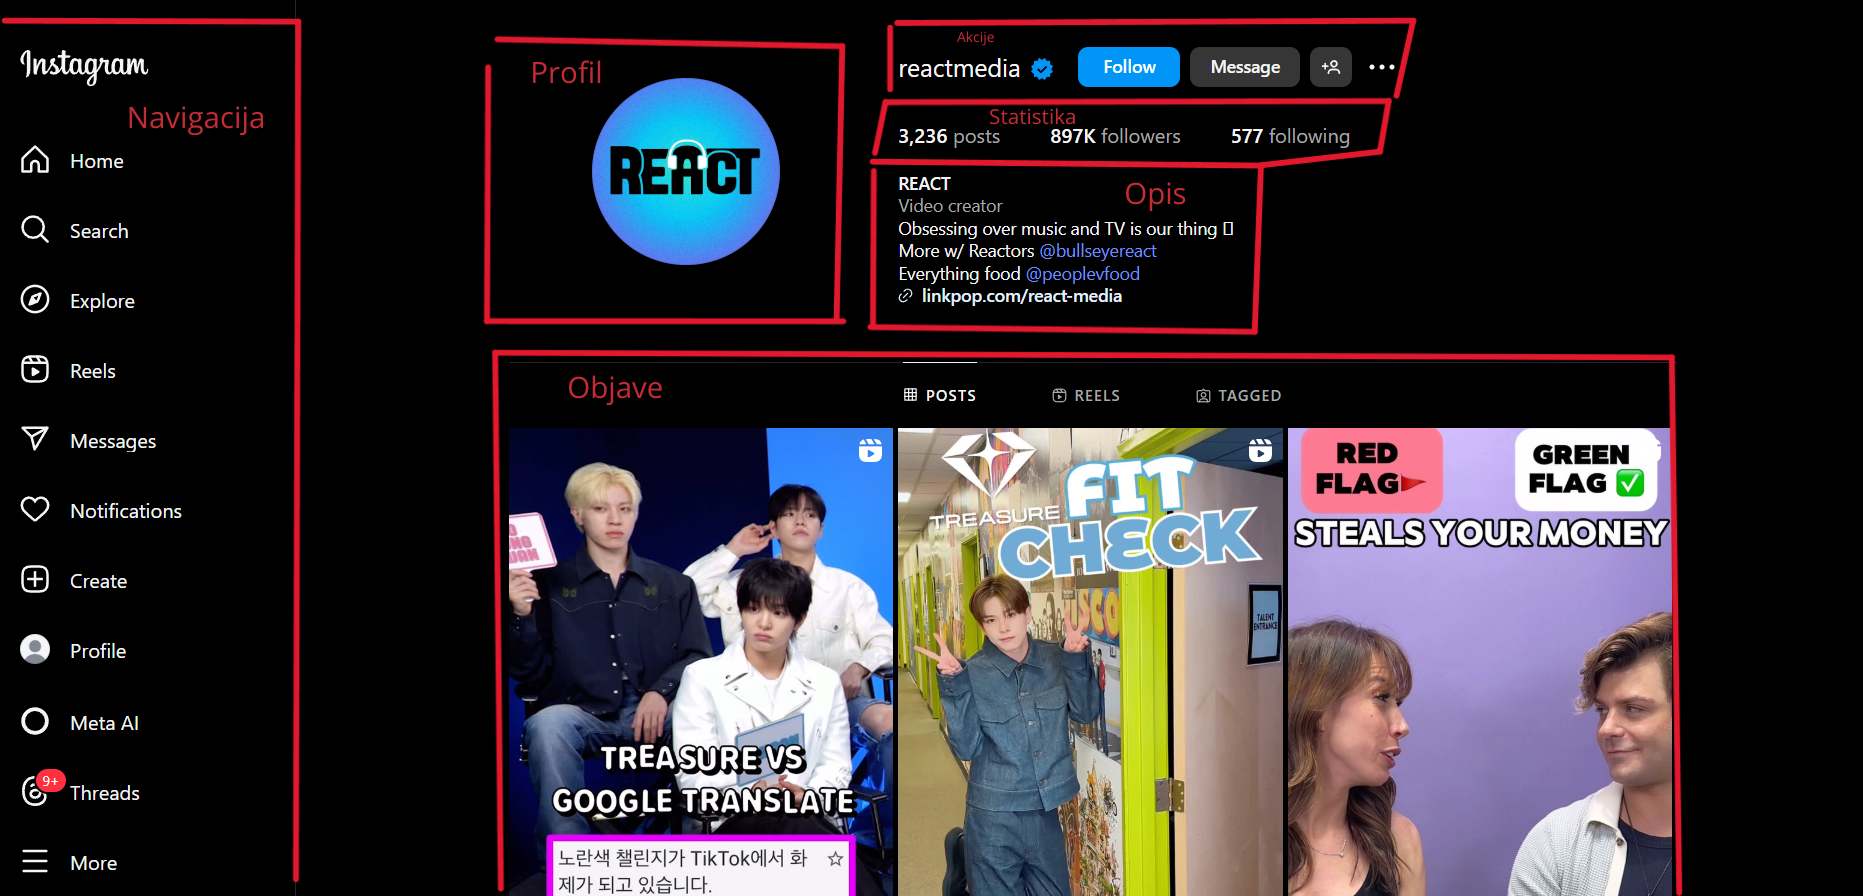
\includegraphics[width=0.6\textwidth]{./assets/components.png} 
    \caption{React komponenta}
    \label{fig:slika5}
\end{figure}


Jedna zanimljivost vezana uz React programere, promatrana na dvije potpuno različite lokacije, otkriva da su indijski developeri za isti posao plaćeni i do deset puta manje (podaci za 2021. godinu). 
To jasno odražava razliku u životnom standardu i ekonomskim potrebama pojedinih zemalja \cite{simplilearn2025react}.
\begin{itemize}
    \item Prosječna plaća za početnog React developera u SAD-u iznosi oko 87000 USD godišnje,
    \item Prosječna plaća za početnog React developera u Indiji iznosi oko 8000 USD godišnje.
\end{itemize}

\section{SMTP}
SMTP (eng. Simple Mail Transfer Protocol) je TCP/IP protokol koji se koristi za slanje i primanje epošte preko mreže kao što je internet.
Neki od primjera klijenata koji koriste SMTP su Gmail, Microsoft Outlook, Yahoo Mail i Apple Mail \cite{gillisSMTP}. 

\begin{figure}[ht!]
    \centering
    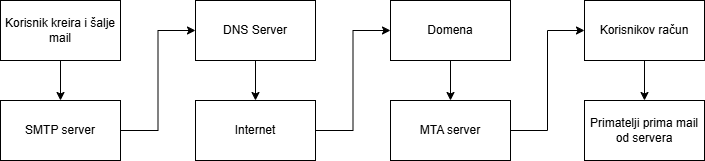
\includegraphics[width=0.8\textwidth]{./assets/Proces dostavljanja emaila.png} 
    \caption{Proces dostavljanja emaila; \href{https://www.techtarget.com/rms/onlineimages/email_delivery_process-f.png}{Izvor}}
    \label{fig:slika17}
\end{figure}

Prethodna slika prikazuje proces slanje epošte kroz SMTP protokol. Proces se odvija prema sljedećim koracima \cite{gillisSMTP}:
\begin{enumerate}
    \item Korisnik piše i šalje email npr. putem web aplikacije,
    \item Email odlazi na SMTP poslužitelj koji je konfiguriran za primanje poruka i njihovo prosljeđivanje,
    \item Nakon toga SMTP server kontaktira DNS server kako bi pronašao IP adresu poslužitelja primatelja. DNS prevodi adresu e-mail domene u IP adresu,
    \item Kada se sazna gdje poruka ide, ona putuje kroz internet prema odredišnom serveru,
    \item Email stiže na domenu primatelja i njen MTA (eng. Mail Transfer Agent) poslužitelj, koji prima poruku i pohranjuje u korisnikov sandučić,
    \item Email je pohranjen na serveru primatelja i čeka da ga korisnik preuzme,
    \item Primatelj može dohvatiti poruku putem IMAP (ostaje na serveru, pristup s više uređaja) ili POP (skida se lokalno, briše se sa servera) načina.
\end{enumerate}
\newpage
\section{FastAPI}
FastAPI je moderan, brz, visokoučinkovit web framework za izgradnju API-ja s Pythonom. Vrlo je brz (u rangu s NodeJS-om i Go-om) i
omogućuje brzo kodiranje i pojavljivanje manjeg broja grešaka. Dosta je intuitivan i jednostavan za korištenje i učenje. FastAPI podržava CRUD
(eng. Create, Read, Update, Delete) operacije koje je moguće koristiti kroz ključne riječi HTTP metoda (GET, POST, PUT, DELETE). Za pokretanje
FastAPI koristi port 8000 i može se testirati putem preglednika ili alata poput Postmana. 8000/docs putanja omogućuje pristup
Swagger UI sučelju koje omogućuje pregled i testiranje API-ja \cite{obafemi2025fastapi}. 


\chapter{Praktični dio rada}
Praktični dio rada se sastoji od izrade web stranice i izrade inteligentnog asistenta temeljenog na RAG tehnologiji. Frontend aplikacije
je izrađen pomoću biblioteke React, pri čemu je korisničko sučelje strukturirano korištenjem JSX sintakse. Backend aplikacije razvijen je korištenjem Python web frameworka FastAPI, 
koji je poznat po svojoj jednostavnosti korištenja. Za izradu inteligentnog asistenta napravljen je scraper podataka s kojim je izrađen skup podataka koji je poslužio za rad inteligentnog
asistenta.

\begin{figure}[ht!]
    \centering
    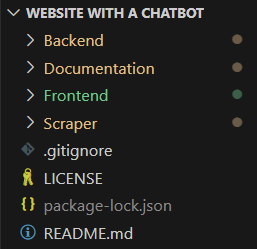
\includegraphics[width=0.25\textwidth]{./assets/Structure-main.png} 
    \caption{Struktura praktičnog dijela rada}
    \label{fig:slika180}
\end{figure}

Struktura praktičnog dijela organizirana je na način da postoje 4 glavna dijela: backend, frontend, scraper i dokumentacija. Ideja ovakvog
pristupa je da sve što je vezano za ovaj rad bude dostupno na jednom mjestu, čime se olakšava razumijevanje ovog rada. Prije početka rada potrebno je instalirati Python, NodeJS + npm, beautifulsoup4, fastapi, uvicorn, langchain, openai i requests.

Za instalaciju i konfiguraciju LaTeX-a u lokalnom okruženju unutar VS Code-a koristan je bio sljedeći video \url{https://www.youtube.com/watch?v=4lyHIQl4VM8}. Za prikaz koda u dokumentu
korištena je biblioteka minted, koja omogućuje sintaksno obojeni ispis izvornog koda. Budući da minted koristi vanjski program pygmentize, potrebno je omogućiti --shell-escape prilikom 
kompilacije. To se postiže izmjenom postavki u datoteci settings.json, gdje se dodaje odgovarajuća konfiguracija. CTRL + Shift + P (za otvaranje prozora).

\begin{longlisting}
\begin{minted}[
    bgcolor=codebg,
    linenos,
    fontsize=\footnotesize,
    breaklines,
    breakanywhere,
    baselinestretch=1.0
]{JSON}
{
  "explorer.confirmDelete": false,
  "php.validate.executablePath": "",
  "latex-workshop.latex.tools": [{
      "name": "pdflatex",
      "command": "pdflatex",
      "args": [
        "--shell-escape",
        "-interaction=nonstopmode",
        "-synctex=1",
        "%DOC%"
      ]}],
  "latex-workshop.latex.recipes": [{
      "name": "pdflatex",
      "tools": ["pdflatex"]
    }]
}
\end{minted}
\caption{settings.json}
\label{lst:settings}
\end{longlisting}

\newpage


\section{Struktura web stranice}
Sljedeća tablica prikazuje pregled stranica web aplikacije te pripadajuće komponente koje su na njima implementirane. Svaka stranica ima svoju
svrhu čime se osigurava intuitivna navigacija. 
\begin{table}[ht!]
\centering
\caption{Struktura stranica i njihovih komponenti}
\renewcommand{\arraystretch}{1.4}
\begin{tabular}{|p{3.5cm}|p{5cm}|p{6.2cm}|}
\hline
\textbf{Stranica / Element} & \textbf{Komponente} & \textbf{Opis} \\
\hline
Početna & Slider, Motivacija, Kratko o Łódźu, Drugi gradovi & Uvodna stranica s informacijama i poveznicama prema ostalim dijelovima stranice. \\
\hline
O Łódźu & Dodatno o gradu, Iskustva bivših studenata & Informacije o gradu i iskustvima Erasmus+ studenata. \\
\hline
Drugi gradovi & Pregled gradova & Pregled ostalih gradova Poljske koje je moguće posjetit. \\
\hline
Pitanja & Forma za postavljanje pitanja & Korisnik postavlja pitanje ako AI asistent ne ponudi tražene informacije. \\
\hline
Dokumenti & Pregled, dodavanje i brisanje dokumenata za RAG & Sekcija za prikaz i pregled dokumenata koji služe kako bi se odgovorilo na pitanja korisnika. \\
\hline
AI asistent (pop-up) & Sučelje za razgovor & Interaktivni chat s korisnikom; otvara se klikom na ikonu asistenta. \\
\hline
\end{tabular}
\end{table}

\textbf{[Napomena]} - Svaka stranica sadrži obavezne elemente kao što su podnožje (eng. footer) i zaglavlje (eng. header).

\section{Korisničko sučelje (Frontend)}
Na sljedećoj slici može se vidjeti struktura frontend dijela. Prikazane su samo određeni dijelovi koji predstavljaju najvažnije
stvari u frontend dijelu.
\begin{figure}[ht!]
    \centering
    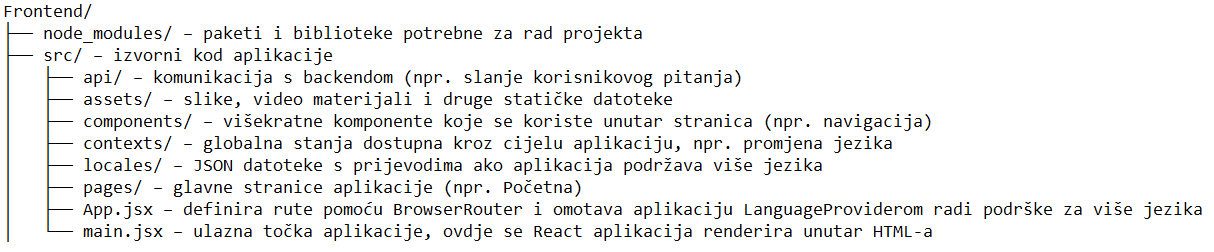
\includegraphics[width=0.9\textwidth]{./assets/frontendstructure.png} 
    \caption{Struktura frontend dijela}
    \label{fig:slika18}
\end{figure}

U okviru frontend dijela prikazani su samo odabrani dijelovi koda i komponente zbog njihove opsežnosti. U slučaju interesa za konkretnim dijelom, izvorni kod je dostupan na Github 
repozitoriju koji je naveden u zaključku rada.

Funkcija askAssistant šalje pitanje i opcionalno PDF datoteke backendu putem HTTP POST zahtjeva. Koristi se za komunikaciju s FastAPI-jem
(ruta /ask) koji obrađuje pitanje uz kontekst PDF-ova.

\begin{longlisting}
\begin{minted}[
    bgcolor=codebg,
    linenos,
    fontsize=\footnotesize,
    breaklines,
    breakanywhere,
    baselinestretch=1.0
]{JavaScript}
export async function askAssistant(question, files = []) {
    const formData = new FormData();
    formData.append("question", question);

    if (files && files.length > 0) {
        files.forEach(file => formData.append("pdfs", file));
    }

    const response = await fetch("http://localhost:8000/ask", {
        method: "POST",
        body: formData,
    });

    if (!response.ok) {
        throw new Error(`Request failed: ${response.statusText}`);
    }

    const data = await response.json();
    return data;
}
\end{minted}
\caption{Chat.jsx}
\label{lst:chat}
\end{longlisting}

Funkcija sendContactForm šalje podatke iz kontakt forme na backend rutu /send email koristeći POST zahtjev s JSON tijelom.
Koristi se za slanje emailova s korisničkim podacima (ime, email, poruka itd.) na server putem FastAPI endpointa.


\begin{longlisting}
\begin{minted}[
    bgcolor=codebg,
    linenos,
    fontsize=\footnotesize,
    breaklines,
    breakanywhere,
    baselinestretch=1.0
]{JavaScript}
export async function sendContactForm(formData) {
  const response = await fetch("http://localhost:8000/send-email", {
    method: "POST",
    headers: {
      "Content-Type": "application/json",
    },
    body: JSON.stringify(formData),
  });

  if (!response.ok) {
    const data = await response.json();
    throw new Error(data.error || "Greška prilikom slanja e-maila.");
  }

  return response.json();
}
\end{minted}
\caption{Contact.jsx}
\label{lst:contact}
\end{longlisting}


\section{Poslužiteljski dio (Backend)}
Na sljedećoj slici može se vidjeti struktura backend dijela. Prikazane su sve stvari koje su od značaja za backend dio aplikacije.
\begin{figure}[ht!]
    \centering
    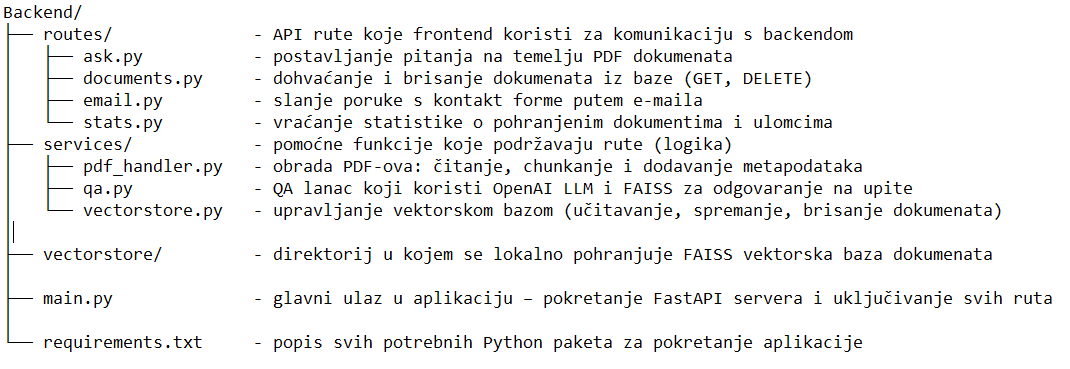
\includegraphics[width=1\textwidth]{./assets/backendstructure.png}
    \caption{Struktura backend dijela}
    \label{fig:slika111}
\end{figure}

Env datoteka sadrži konfiguracijske varijable koje se koriste u aplikaciji. OpenAI API ključ se koristi za pristup OpenAI modelima,
Gmail user je adresa s koje se šalju poruke s kontakt forme, Gmail password je aplikacijska lozinka za autentifikaciju Gmail računa i Gmail receiver
je adresa primatelja poruka koja može biti kao Gmail user.

\begin{figure}[h]
  \centering
  
\includegraphics[width=0.5\textwidth]{./assets/env file.png}
  \caption{Sadržaj env datoteke}
  \label{fig:slika121}
\end{figure}


\subsection{Server}
Main predstavlja glavnu datoteku koja pokreće FastAPI aplikaciju. Učitava se konfiguracija iz .env datoteke, omogućuje se CORS pristup
kako bi frontend i backend mogli komunicirati bez ograničenja, te se u aplikaciju uključuju sve definirane rute za pitanja, dokumente, statistiku
i email. 

\begin{longlisting}
\begin{minted}[
    bgcolor=codebg,
    linenos,
    fontsize=\footnotesize,
    breaklines,
    breakanywhere,
    baselinestretch=1.0
]{Python}
from fastapi import FastAPI
from fastapi.middleware.cors import CORSMiddleware
from dotenv import load_dotenv

from routes import ask, documents, stats, email

load_dotenv()

app = FastAPI()

app.add_middleware(
    CORSMiddleware,
    allow_origins=["*"],
    allow_credentials=True,
    allow_methods=["*"],
    allow_headers=["*"],
)

app.include_router(ask.router)
app.include_router(documents.router)
app.include_router(stats.router)
app.include_router(email.router)

\end{minted}
\caption{Main.py}
\label{lst:main}
\end{longlisting}


\subsection{Servisi}

Sljedeći dio koda upravlja vektorskom bazom podataka koristeći FAISS i OpenAIEmbeddings. Omogućuje učitavanje vektorske baze podataka, dodavanje
novih dokumenata te brisanje dokumenata na temelju imena datoteke. Vektorska baza podataka se lokalno pohranjuje u direktorij vectorstore.

\begin{longlisting}
\begin{minted}[
    bgcolor=codebg,
    linenos,
    fontsize=\footnotesize,
    breaklines,
    breakanywhere,
    baselinestretch=1.0
]{Python}
import os
from langchain_community.embeddings import OpenAIEmbeddings
from langchain_community.vectorstores import FAISS

VECTORSTORE_DIR = "vectorstore"

def load_vectorstore():
    embeddings = OpenAIEmbeddings()
    if not os.path.exists(VECTORSTORE_DIR):
        raise FileNotFoundError("Vectorstore not found.")
    return FAISS.load_local(VECTORSTORE_DIR, embeddings, allow_dangerous_deserialization=True)

def get_or_create_vectorstore(all_docs):
    embeddings = OpenAIEmbeddings()

    if os.path.exists(VECTORSTORE_DIR):
        db = FAISS.load_local(VECTORSTORE_DIR, embeddings, allow_dangerous_deserialization=True)
        if all_docs:
            db.add_documents(all_docs)
            db.save_local(VECTORSTORE_DIR)
    elif all_docs:
        db = FAISS.from_documents(all_docs, embeddings)
        db.save_local(VECTORSTORE_DIR)
    else:
        raise ValueError("No documents provided and vectorstore doesn't exist.")

    return db

def delete_file_from_vectorstore(filename):
    try:
        db = load_vectorstore()
    except FileNotFoundError:
        return False

    remaining_docs = [
        doc for doc in db.docstore._dict.values()
        if doc.metadata.get("source") != filename
    ]

    if len(remaining_docs) == len(db.docstore._dict):
        return False

    embeddings = OpenAIEmbeddings()
    new_db = FAISS.from_documents(remaining_docs, embeddings)
    new_db.save_local(VECTORSTORE_DIR)
    return True
\end{minted}
\caption{Vectorstore.py}
\label{lst:vectorstore}
\end{longlisting}

Nadalje se definira mehanizam za dohvaćanje odgovora na pitanja pomoću modela gpt-3.5-turbo-16k i prethodno izgrađene vektorske baze.
Koristi se RetrievalQA lanac koji kombinira jezični model s retriverom za dohvat relevantnih dokumenata. Može se podesiti broj dokumenata
koji se koriste za generiranje odgovora.
\begin{longlisting}
\begin{minted}[
    bgcolor=codebg,
    linenos,
    fontsize=\footnotesize,
    breaklines,
    breakanywhere,
    baselinestretch=1.0
]{Python}
from langchain_openai import ChatOpenAI
from langchain.chains import RetrievalQA

def get_qa_chain(db):
    retriever = db.as_retriever(search_kwargs={"k": 2}) 
    llm = ChatOpenAI(model="gpt-3.5-turbo-16k")
    return RetrievalQA.from_chain_type(llm=llm, retriever=retriever)
\end{minted}
\caption{qa.py}
\label{lst:qa}
\end{longlisting}

\subsection{Rute}
Ova API ruta omogućuje korisniku da pošalje jedan ili više PDF dokumenata i postavit pitanje vezano uz njihov sadržaj. PDF dokumenti
se obrađuju i dijele na manje dijelove, a zatim se kreira ili nadopunjuje vektorska baza podataka. Jezični model koristi najrelevantnije dijelove
za generiranje odgovora. Ruta vraća generirani odgovor zajedno s porukom o uspješnoj obradi i indeksiranju PDF dokumenata.

\begin{longlisting}
\begin{minted}[
    bgcolor=codebg,
    linenos,
    fontsize=\footnotesize,
    breaklines,
    breakanywhere,
    baselinestretch=1.0
]{Python}
from fastapi import APIRouter, UploadFile, File, Form
from services.pdf_handler import process_pdfs
from services.vectorstore import get_or_create_vectorstore
from services.qa import get_qa_chain

router = APIRouter()

@router.post("/ask")
async def ask_pdf(
    question: str = Form(...),
    pdfs: list[UploadFile] = File(None)
):
    all_docs = await process_pdfs(pdfs)
    db = get_or_create_vectorstore(all_docs)
    qa_chain = get_qa_chain(db)
    response = qa_chain.run(question)

    return {"answer": response, "message": "PDF document successfully added and indexed."}
\end{minted}
\caption{ask.py}
\label{lst:ask}
\end{longlisting}

Nadalje su definirane dvije rute: jedna za dohvat popisa svih PDF dokumenata koji su trenutno indeksirani u vektorskoj bazi podataka, a druga
za brisanje dokumenata po nazivu dokumenta. Ruta za brisanje vraća grešku ako dokument s tim imenom ne postoji u vektorskoj bazi podataka.

\begin{longlisting}
\begin{minted}[
    bgcolor=codebg,
    linenos,
    fontsize=\footnotesize,
    breaklines,
    breakanywhere,
    baselinestretch=1.0
]{Python}
from fastapi import APIRouter, HTTPException
from services.vectorstore import load_vectorstore, delete_file_from_vectorstore

router = APIRouter()

@router.get("/documents")
def list_documents():
    db = load_vectorstore()
    sources = set()
    for doc in db.docstore._dict.values():
        if "source" in doc.metadata:
            sources.add(doc.metadata["source"])
    return {"documents": list(sources)}

@router.delete("/delete-document")
def delete_document(filename: str):
    success = delete_file_from_vectorstore(filename)
    if not success:
        raise HTTPException(status_code=404, detail=f"No document found with source: {filename}")
    return {"status": "success", "message": f"Deleted document: {filename}"}
\end{minted}
\caption{documents.py}
\label{lst:documents}
\end{longlisting}

Sljedeća API ruta omogućuje slanje e-mail poruke s kontakt forme. Korisnik ispunjava ime, email, broj telefona, adresu i poruku, a backend
zatim šalje e-mail na zadanu adresu koristeći Gmail SMTP. Podaci se šalju putem SSL-a, a konfiguracija dolazi iz .env datoteke.

\begin{longlisting}
\begin{minted}[
    bgcolor=codebg,
    linenos,
    fontsize=\footnotesize,
    breaklines,
    breakanywhere,
    baselinestretch=1.0
]{Python}
from fastapi import APIRouter
from pydantic import BaseModel, EmailStr
import smtplib
from email.mime.text import MIMEText
from email.utils import formataddr
from dotenv import load_dotenv
import os

load_dotenv()

router = APIRouter()

class ContactForm(BaseModel):
    fullName: str
    phone: str
    email: EmailStr
    address: str
    description: str

@router.post("/send-email")
def send_email(data: ContactForm):
    sender_email = os.getenv("GMAIL_USER")
    sender_password = os.getenv("GMAIL_PASSWORD")
    receiver_email = os.getenv("GMAIL_RECEIVER") or sender_email

    msg_content = f"""
    Nova poruka s kontakt forme:

    Ime i prezime: {data.fullName}
    Telefon: {data.phone}
    E-mail: {data.email}
    Adresa: {data.address}
    Poruka:
    {data.description}
    """

    msg = MIMEText(msg_content, "plain", "utf-8")
    msg["Subject"] = "Nova poruka s web stranice"
    msg["From"] = formataddr(("Web kontakt forma", sender_email))
    msg["To"] = receiver_email
    msg["Reply-To"] = data.email  

    try:
        with smtplib.SMTP_SSL("smtp.gmail.com", 465) as server:
            server.login(sender_email, sender_password)
            server.sendmail(sender_email, receiver_email, msg.as_string())
        return {"message": "Email je uspješno poslan."}
    except Exception as e:
        print("Greška prilikom slanja emaila:", e)
        return {"error": "Neuspješno slanje emaila. Provjerite postavke."}
\end{minted}
\caption{email.py}
\label{lst:email}
\end{longlisting}


\subsection{Inteligentni asistent}
test
\subsubsection{Prikupljanje podataka}

Prikupljanje podataka započelo je kroz razgovor s profesoricom umjetne inteligencije koju sam upoznao tijekom Erasmus+ razmjene. 
Profesorica je bila izuzetno korisna osoba za ovaj rad jer je rođena i živi u gradu Łódź. Ukratko sam joj predstavio temu rada, 
a ona mi je preporučila nekoliko relevantnih internetskih izvora.

Sljedeća tablica prikazuje pregled korištenih izvora, broj zapisa, naziv rezultirajuće datoteke i alate korištene za obradu podataka:

\begin{table}[H]
\centering
\begin{tabular}{|p{4cm}|p{3.5cm}|p{5cm}|p{3.5cm}|}
\hline
\textbf{Web izvor} & \textbf{Veličina skupa podataka} & \textbf{Naziv datoteke} & \textbf{Korišteni alati} \\
\hline
\url{https://lodz.pl/} & 1000 zapisa & \raggedright\texttt{lodz\_articles} & \texttt{scraper2.py}, \texttt{translator.py} \\
\hline
\url{https://lodz.travel/turystyka/co-zobaczyc/} & 185 zapisa & \raggedright\texttt{lodz\_destinations} & \texttt{scraper.py}, \texttt{translator.py} \\
\hline
\url{https://polskapogodzinach.pl/lodz-atrakcje/} & 52 stranice & \raggedright\texttt{lodz\_attractions} & ručno konvertirano u PDF \\
\hline
\end{tabular}
\caption{Korišteni izvori podataka i alati za obradu}
\label{tab:izvori}
\end{table}



\subsubsection{Web scraping}
\begin{figure}[ht!]
    \centering
    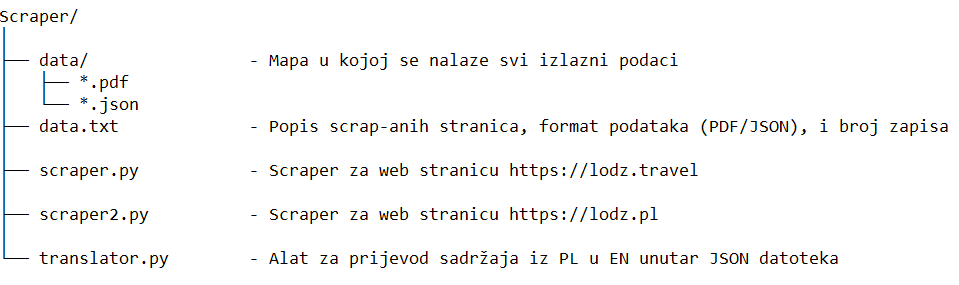
\includegraphics[width=1\textwidth]{./assets/structure-scraper.png}
    \caption{Struktura scraper foldera}
    \label{fig:slika1111}
\end{figure}

Sljedeća metoda dohvaća HTML sadržaj stranice. Prima URL i vraća BeautifulSoup objekt za lakšu obradu HTML-a. Postavlja User-Agent 
kako bi se izbjeglo blokiranje od strane servera. U slučaju do pogreške (npr. timeout) ispisuje poruku i vraća None. 

\begin{longlisting}
\begin{minted}[
    bgcolor=codebg,
    linenos,
    fontsize=\footnotesize,
    breaklines,
    breakanywhere,
    baselinestretch=1.0
]{python}
import requests
from bs4 import BeautifulSoup
from urllib.parse import urljoin
import json
import time

BASE_URL = "https://lodz.travel"
visited_urls = set()

def get_soup(url):
    print(f"Fetching: {url}")
    try:
        res = requests.get(url, headers={
            "User-Agent": "Mozilla/5.0"
        })
        res.encoding = 'utf-8'
        return BeautifulSoup(res.text, 'html.parser')
    except Exception as e:
        print(f"Error fetching page: {e}")
        return None
\end{minted}
\caption{Scraper 1/6}
\label{lst:scraper1}
\end{longlisting}

Ova metoda rekurzivno prolazi kroz listu i sve li stavke u njoj. Za svaku pronađenu stranicu iz izbornika izdvaja se title i href te se stvara
struktura koja sadrži title, url, content i subcategories.

\begin{longlisting}
\begin{minted}[
    bgcolor=codebg,
    linenos,
    fontsize=\footnotesize,
    breaklines,
    breakanywhere,
    baselinestretch=1.0
]{python}
def parse_menu(ul_tag, level=1):
    data = []
    for li in ul_tag.find_all("li", recursive=False):
        a_tag = li.find("a", recursive=False)
        if not a_tag:
            continue
        title = a_tag.text.strip()
        href = urljoin(BASE_URL, a_tag["href"])
        print(f"{'  ' * (level-1)}({level}) {title} -> {href}")
        node = {
            "title": title,
            "url": href,
            "content": "",
        }
        sub_ul = li.find("ul")
        if sub_ul:
            node["subcategories"] = parse_menu(sub_ul, level + 1)
        data.append(node)
    return data
\end{minted}
\caption{Scraper 2/6}
\label{lst:scraper2}
\end{longlisting}

Sljedeća metoda dohvaća sadržaj za svaku stranicu. Ulazi u svaku stranicu u hijerarhiji i izdvaja tekst iz diva s klasom ce-bodytext.
Sprema pročišćeni tekst u item["content"] te traži dodatne poveznice unutar sadržaja i dodaje ih kao subcategories i rekurzivno ih obađuje.


\begin{longlisting}
\begin{minted}[
    bgcolor=codebg,
    linenos,
    fontsize=\footnotesize,
    breaklines,
    breakanywhere,
    baselinestretch=1.0
]{python}
def fill_content_recursively(data):
    for item in data:
        if item["url"] in visited_urls:
            continue
        visited_urls.add(item["url"])

        print(f"\nRetrieving content for: {item['title']}")
        soup = get_soup(item["url"])
        if not soup:
            continue

        content_div = soup.select_one("div.ce-bodytext")
        if content_div:
            item["content"] = content_div.get_text(separator="\n", strip=True)
            print(f"Content retrieved successfully ({len(item['content'])} characters)")

            sub_links = []
            for a in content_div.find_all("a", href=True):
                href = urljoin(BASE_URL, a["href"])
                if BASE_URL in href and href not in visited_urls:
                    title = a.get_text(strip=True)
                    if title:
                        sub_links.append({
                            "title": title,
                            "url": href,
                            "content": ""
                        })

            if sub_links:
                print(f"Found {len(sub_links)} internal subpages inside: {item['title']}")
                item["subcategories"] = sub_links
                fill_content_recursively(sub_links)

        if "subcategories" in item:
            fill_content_recursively(item["subcategories"])
\end{minted}
\caption{Scraper 3/6}
\label{lst:scraper3}
\end{longlisting}

Ova metoda broji sve stavke (stranice i podstranice) u hijerarhiji podataka. Koristi se za statistiku na kraju izvršavanja.  

\begin{longlisting}
\begin{minted}[
    bgcolor=codebg,
    linenos,
    fontsize=\footnotesize,
    breaklines,
    breakanywhere,
    baselinestretch=1.0
]{python}
def count_total_items(data):
    count = 0
    for item in data:
        count += 1
        if "subcategories" in item:
            count += count_total_items(item["subcategories"])
    return count
\end{minted}
\caption{Scraper 4/6}
\label{lst:scraper4}
\end{longlisting}

Ova metoda pokreće cijeli proces. Kreće od glavne stranice navigacije gdje se dohvaća struktura linkova pomoću parse menu funkcije.
Zatim se rekurzivno dohvaća sadržaj sa svih stranica pomoću fill content recursively funkcije. Na kraju svi podaci se spremaju u JSON datoteku 
i ispisuje se kolko je ukupno stranica pronađeno i spremljeno.

\begin{longlisting}
\begin{minted}[
    bgcolor=codebg,
    linenos,
    fontsize=\footnotesize,
    breaklines,
    breakanywhere,
    baselinestretch=1.0
]{python}
def main():
    start_url = "https://lodz.travel/turystyka/"
    soup = get_soup(start_url)
    aside_nav = soup.select_one("ul.aside-nav")
    if not aside_nav:
        print("Navigation not found! Check the URL or HTML structure.")
        return

    print("Parsing main navigation...")
    structured_data = parse_menu(aside_nav)

    print("\nFetching content from all pages...")
    fill_content_recursively(structured_data)

    with open("lodz_content.json", "w", encoding="utf-8") as f:
        json.dump(structured_data, f, indent=2, ensure_ascii=False)

    total = count_total_items(structured_data)
    print(f"\nTotal records extracted: {total}")
    print("Done! Data saved to: lodz_content.json")

if __name__ == "__main__":
    main()
\end{minted}
\caption{Scraper 5/6}
\label{lst:scraper5}
\end{longlisting}


Ova python skripta učitava JSON s člancima na poljskom jeziku i prevodi ih na engleski koristeći biblioteku deep-translator. Funkcija rekurzivno pronalazi
kroz sve stavke i podkategorije u JSON strukturi. Napredak prevođenja ispisuje se u konzoli, a prevedeni podaci spremaju se u novu .json
datoteku.
\begin{longlisting}
\begin{minted}[
    bgcolor=codebg,
    linenos,
    fontsize=\footnotesize,
    breaklines,
    breakanywhere,
    baselinestretch=1.0
]{Python}
import json
from deep_translator import GoogleTranslator

INPUT_FILE = "lodz_articles_pl.json"
OUTPUT_FILE = "lodz_articles_en.json"

def translate_text(text, src="pl", target="en"):
    try:
        return GoogleTranslator(source=src, target=target).translate(text)
    except Exception as e:
        return f"[Translation Error] {text}"

def translate_node(node, counter, total):
    if "title" in node:
        node["title"] = translate_text(node["title"])
    if "content" in node and node["content"]:
        node["content"] = translate_text(node["content"])

    counter[0] += 1
    print(f"[{counter[0]}/{total}] translated")

    if "subcategories" in node:
        for sub in node["subcategories"]:
            translate_node(sub, counter, total)

def count_nodes(data):
    count = 0
    for item in data:
        count += 1
        if "subcategories" in item:
            count += count_nodes(item["subcategories"])
    return count

def main():
    print("Loading JSON...")
    with open(INPUT_FILE, "r", encoding="utf-8") as f:
        data = json.load(f)

    total = count_nodes(data)
    print(f"Translating {total} entries...")

    counter = [0] 
    for entry in data:
        translate_node(entry, counter, total)

    print("Saving translated JSON...")
    with open(OUTPUT_FILE, "w", encoding="utf-8") as f:
        json.dump(data, f, ensure_ascii=False, indent=2)

    print(f"Done! Translated file saved as: {OUTPUT_FILE}")

if __name__ == "__main__":
    main()

\end{minted}
\caption{Scraper 6/6}
\label{lst:scraper6}
\end{longlisting}


\subsubsection{Čišćenje i obrada podataka}
test




\newpage
\section{Prikaz rada aplikacije}

Što se tiče frontenda, projekt je razvijan korištenjem Vite okoline, a pokretanje aplikacije omogućeno je korištenjem naredbe \texttt{npm run dev}.

Backend se pokreće lokalno pomoću Uvicorn ASGI servera, korištenjem naredve \texttt{uvicorn main:app --reload} koja omogućuje automatsko
ponovno učitavanje prilikom promjena u kodu.

\begin{figure}[ht]
  \centering
  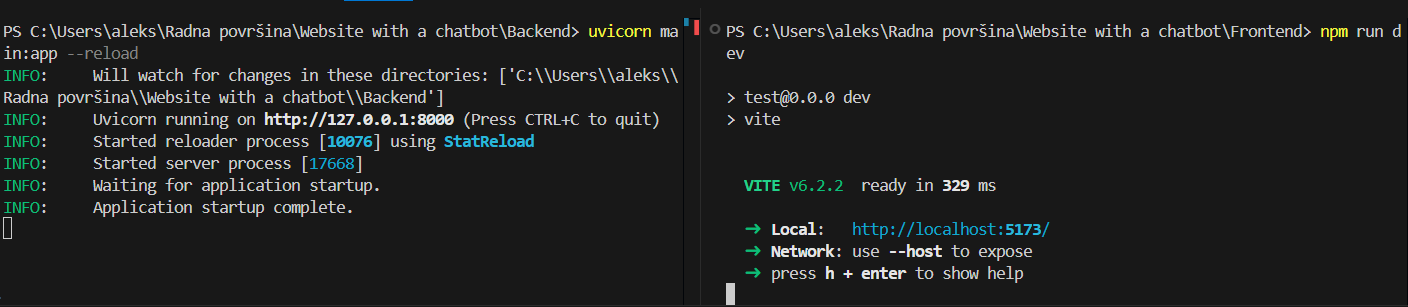
\includegraphics[width=1\textwidth]{./assets/pokretanje.png}
  \caption{Pokretanje aplikacije kroz terminal}
  \label{fig:slika93}
\end{figure}

Sljedeća slika prikazuje početnu stranicu aplikacije na koju se dolazi nakon pokretanja aplikacije. Na početnoj stranici nalazi se nekoliko
komponenta kao što su slider, motivacija, kratko o Łódźu i drugi gradovi. Ideja početne stranice je da korisniku pruži osnovne informacije i odvede
korisnika na ostale stranice aplikacije.

\begin{figure}[ht]
  \centering
  \includegraphics[width=1\textwidth]{./assets/Home.png}
  \caption{Početna stranica aplikacije}
  \label{fig:slika94}
\end{figure}

\newpage

Sljedeća slika prikazuje stranicu O Łódźu koja sadrži dodatne informacije o gradu, uključujući iskustva bivših studenata koji su proveli
Erasmus+ razmjenu u tom gradu.

\begin{figure}[ht]
  \centering
  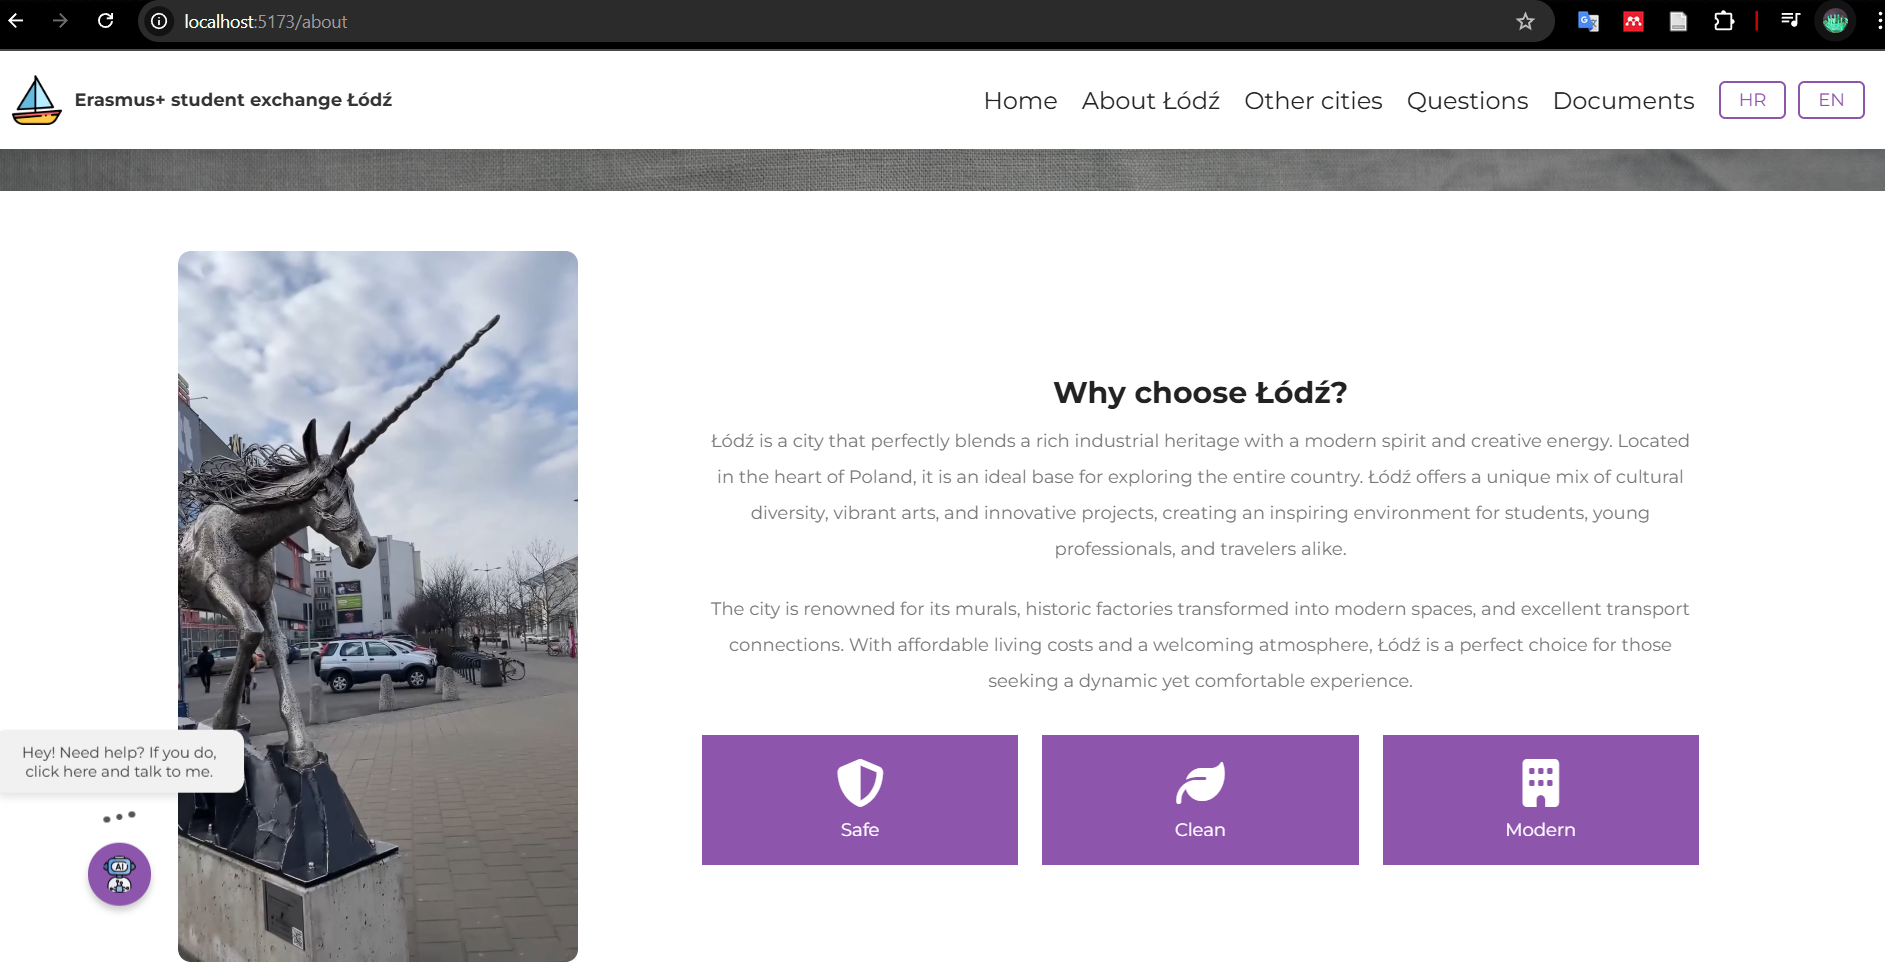
\includegraphics[width=1\textwidth]{./assets/about.png}
  \caption{O Łódźu stranica}
  \label{fig:slika95}
\end{figure}

Stranica drugi gradovi sadrži pregled drugih gradova u Poljskoj koje je moguće posjetiti. Ova stranica pruža korisnicima
informacije u obliku slika i podataka kao što je broj stanovnika.

\begin{figure}[ht]
  \centering
  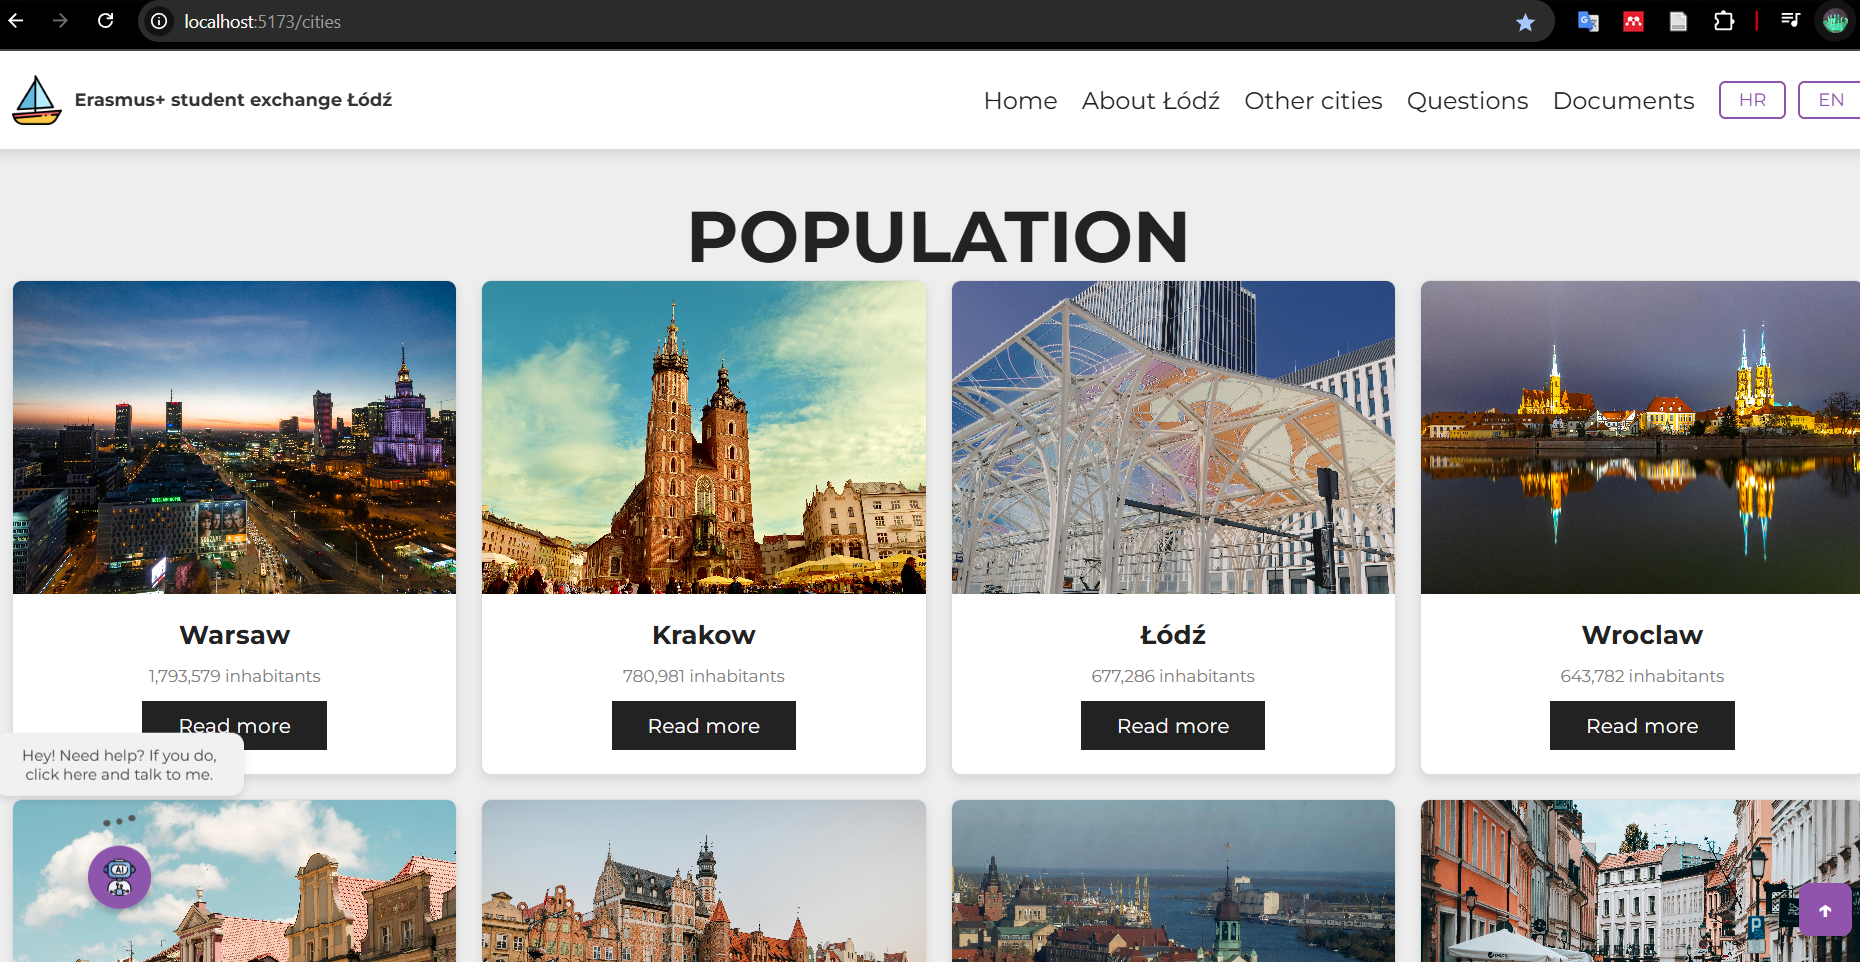
\includegraphics[width=1\textwidth]{./assets/other.png}
  \caption{Drugi gradovi stranica}
  \label{fig:slika96}
\end{figure}

\newpage
Sljedeća stranica namijenjena je za postavljanje pitanja od strane korisnika u slučaju da AI asistent ne pruži odgovor koji korisnik traži.
Nakon slanja odgovora, vlasnik stranice dobiva email s informacijama prema definiranoj formi.

\begin{figure}[ht]
  \centering
  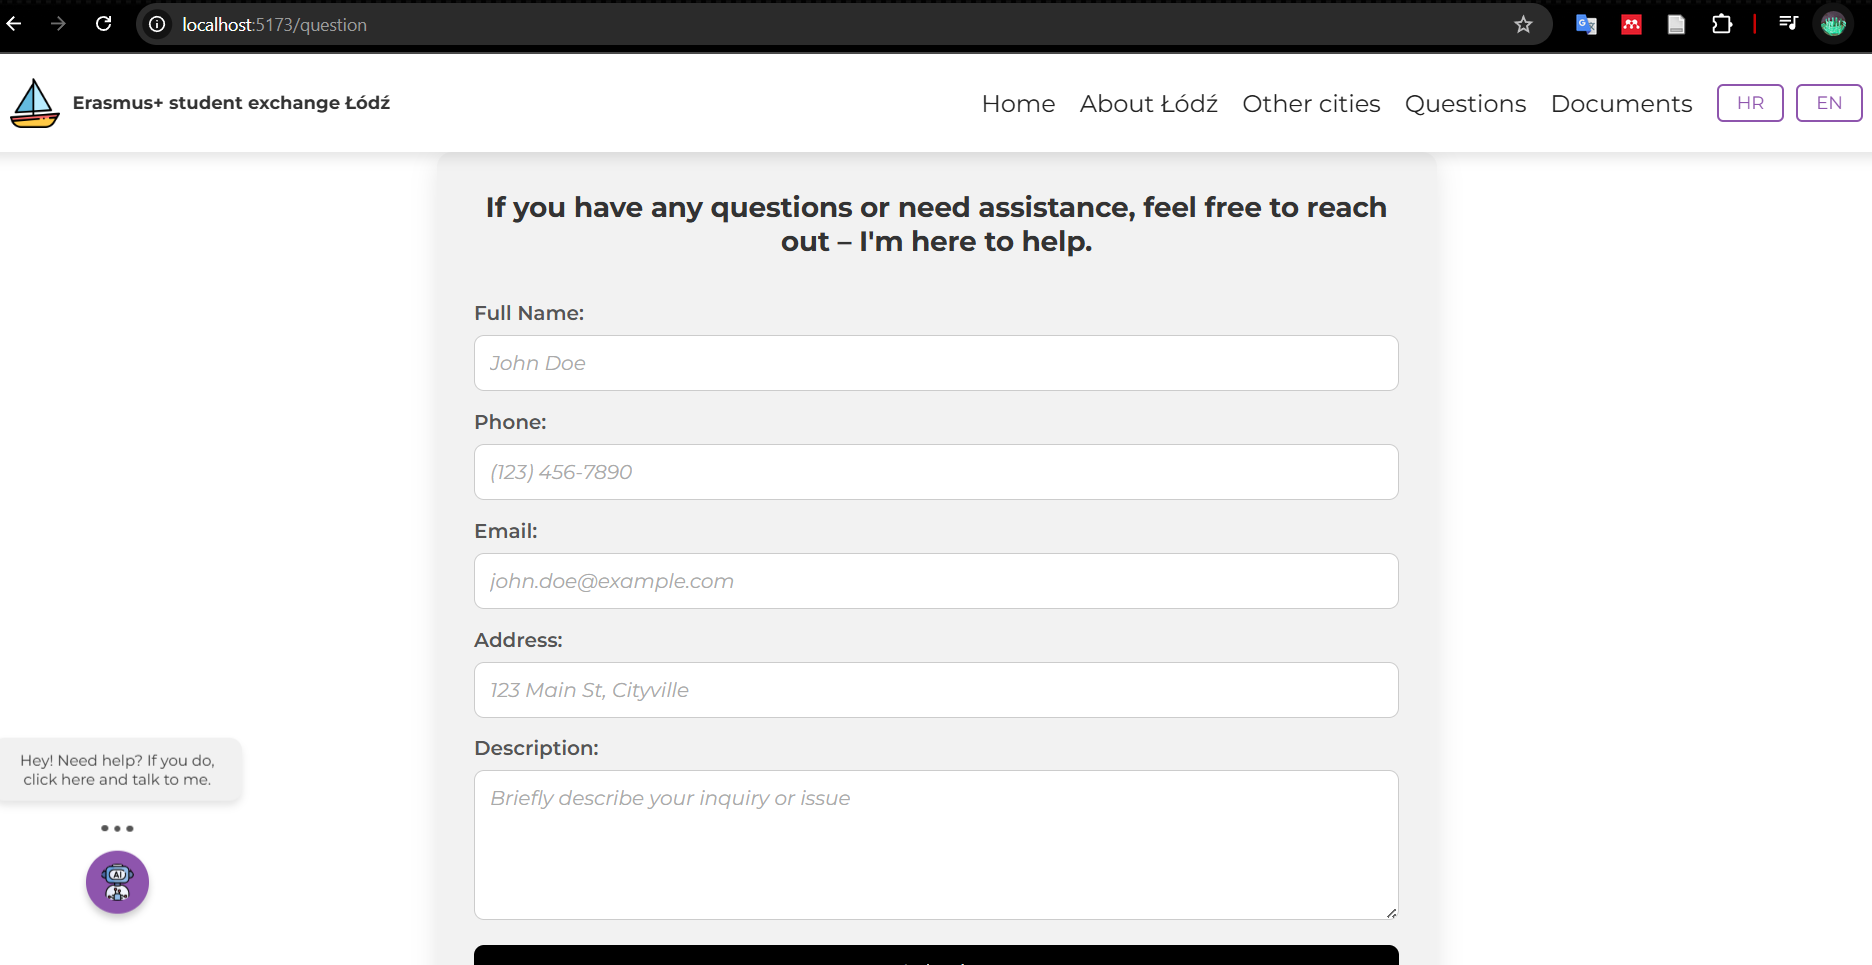
\includegraphics[width=1\textwidth]{./assets/question.png}
  \caption{Forma za postavljanje pitanja stranica}
  \label{fig:slika97}
\end{figure}

Stranica za dokumente omogućuje pregled i upravljanje dokumentima koji se koriste za rad s asistentom. Prvotno ova stranica nije bila U
početnoj ideji rada ali nakon što je započet rad s AI dijelom rada, pojavila se potreba za dodavanjem ove stranice kako bi se bolje 
vizualiziralo što se događa u pozadini rada asistenta.

\begin{figure}[ht]
  \centering
  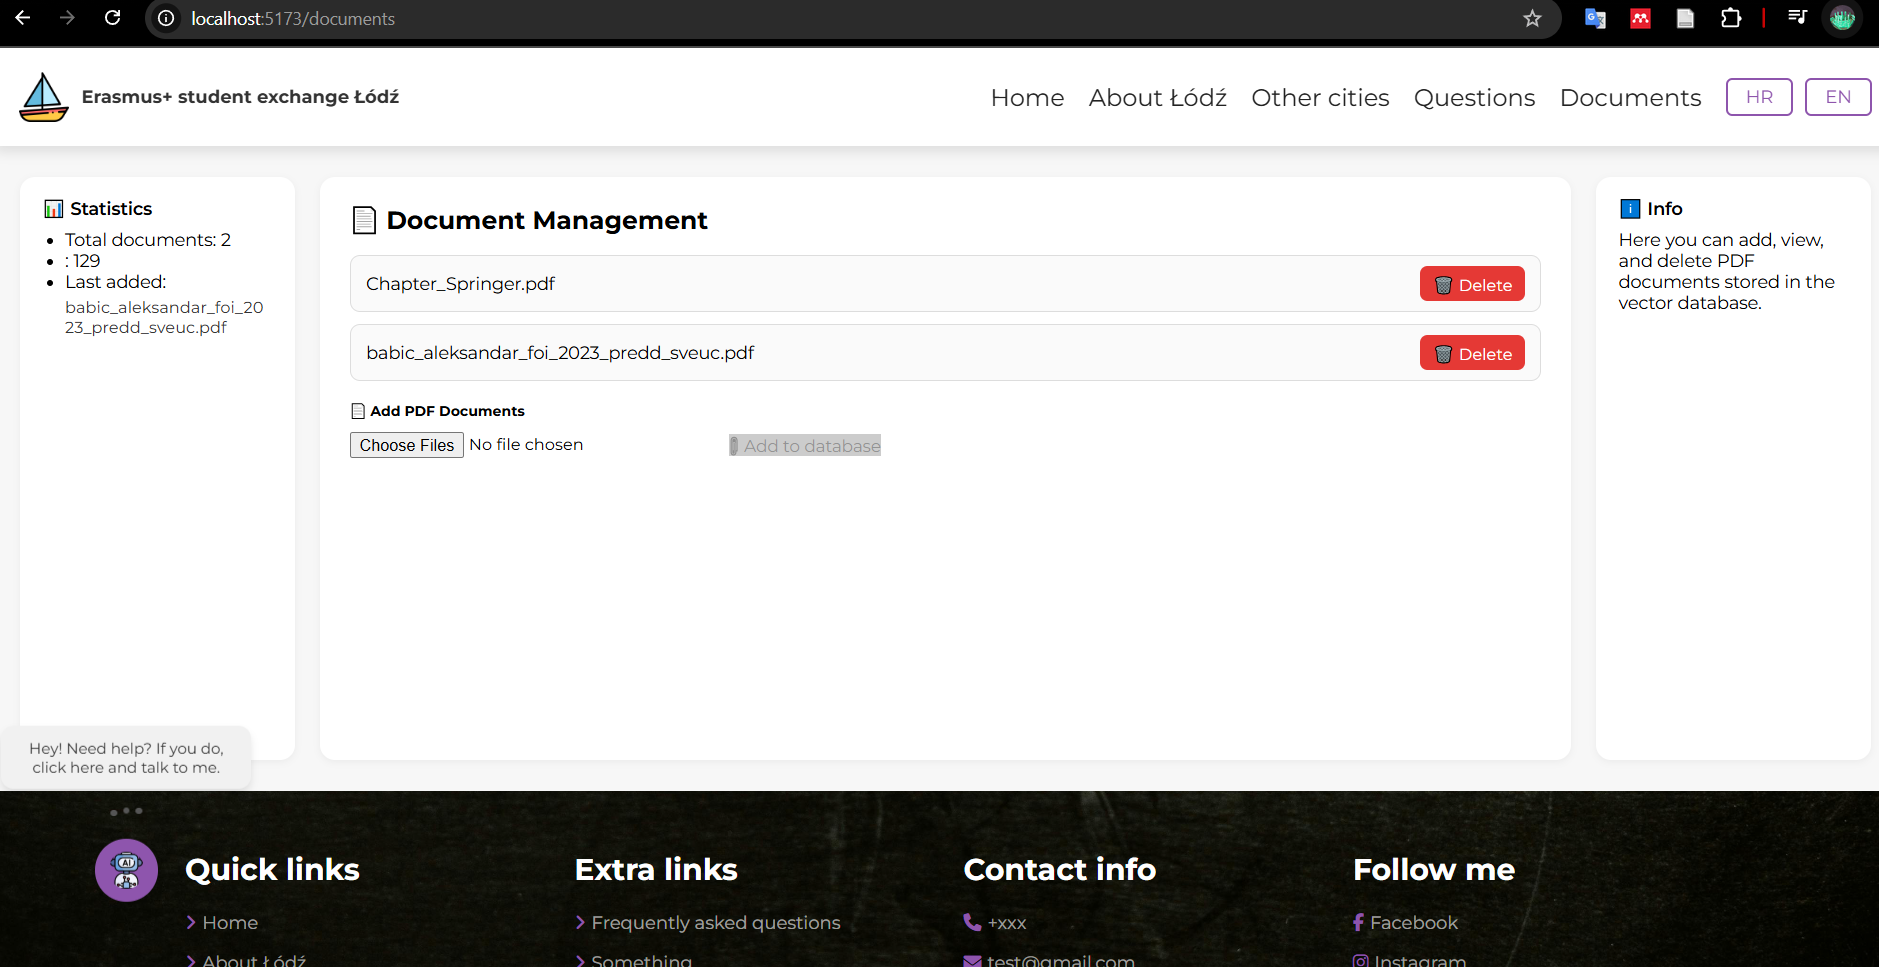
\includegraphics[width=0.9\textwidth]{./assets/documents.png}
  \caption{Stranica za pregled i upravljanje dokumentima}
  \label{fig:slika98}
\end{figure}
\newpage

Na sljedećoj slici može se vidjeti kako funkcionira AI asistent kada je dokument u bazi podataka. Asistent u tom slučaju može odgovoriti na
pitanje korisnika koristeći informacije iz dokumenta.

\begin{figure}[ht]
  \centering
  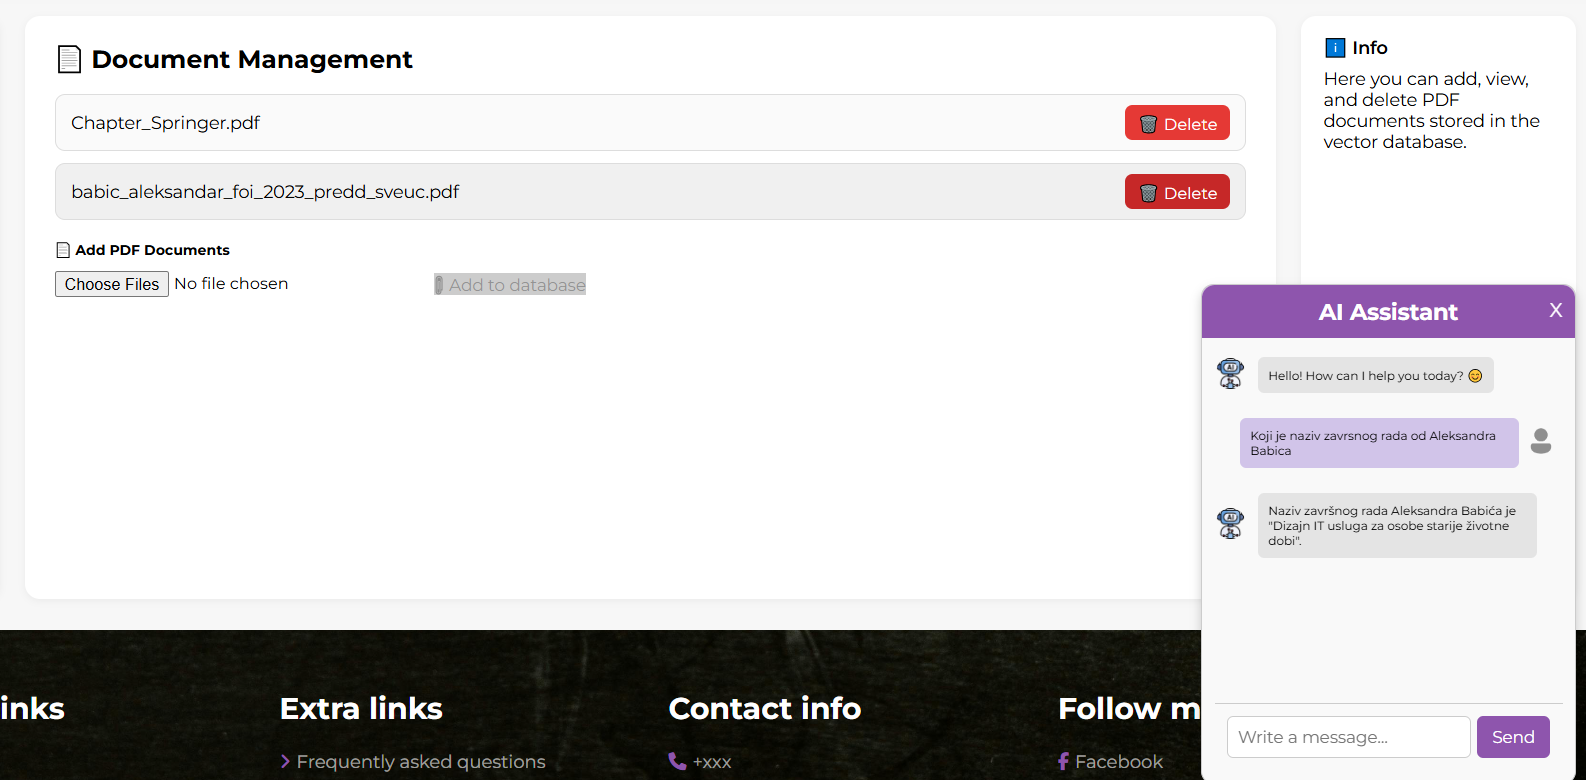
\includegraphics[width=1\textwidth]{./assets/asistent1.png}
  \caption{Testiranje asistenta kada je dokument u bazi}
  \label{fig:slika99}
\end{figure}

Na sljedećoj slici može se vidjeti kako AI asistent reagira kada dokument nije pronađen u bazi podataka.

\begin{figure}[ht]
  \centering
  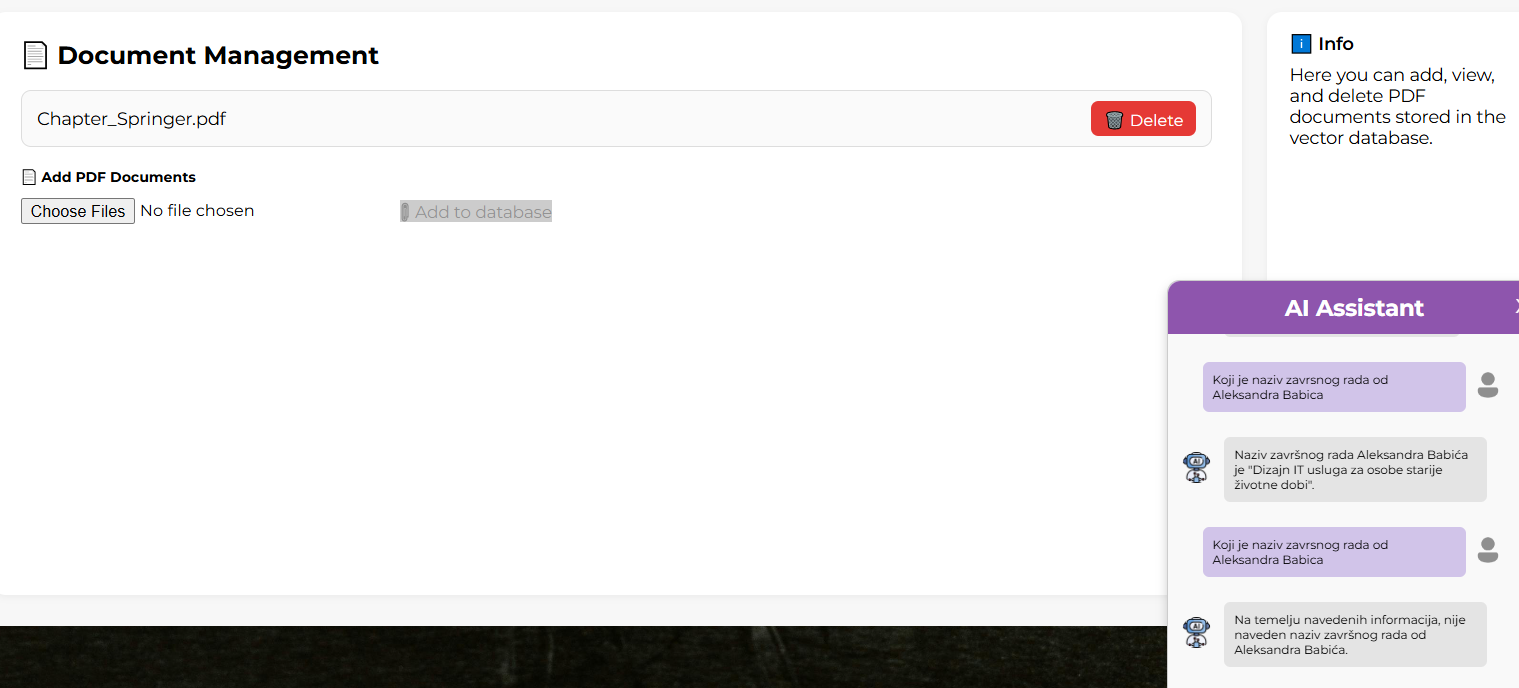
\includegraphics[width=1\textwidth]{./assets/asistent2.png}
  \caption{Testiranje asistenta kad dokument nije u bazi}
  \label{fig:slika100}
\end{figure}
\newpage

Kroz terminal može se vidjeti kako sustav radi u pozadini. Može se vidjeti koji je zahtjev poslan i kakav je status takvog zahtjeva.

\begin{figure}[ht]
  \centering
  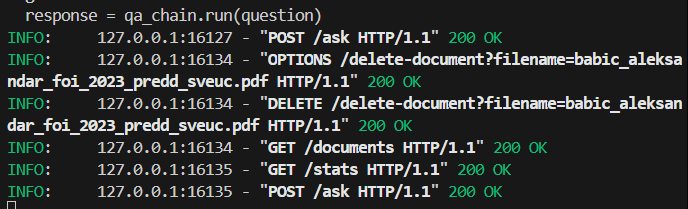
\includegraphics[width=1\textwidth]{./assets/statzs.png}
  \caption{Povratne informacije o radu aplikacije}
  \label{fig:slika101}
\end{figure}

\chapter{Zaključak}











Za kraj, Erasmusa se ne treba bojati jer je to prekasno iskustvo koje se pamti do kraja života. Svaki problem s kojim se suoči osoba, čini osobu jačom i neovisnijom. 
Boravak na jednom mjestu dulje vrijeme postat će čudan način života. Jednom Erasmus+, uvijek Erasmus+!

Poveznica na Github: \href{https://github.com/ababic20/Website-with-a-chatbot.git}{\textbf{Poveznica}} 

\makebackmatter



\end{document}
